\documentclass[preprint,authoryear,12pt]{elsarticle}

\usepackage{amssymb}
\usepackage{amsmath}
\usepackage{graphicx}
%\usepackage{subfigure} Deprecated. This is what Ben originally had. Replaced with subcaption, which is updated, which is what I had in Isles and ESR.
\usepackage{subcaption}
\usepackage{xspace}
\usepackage{bm}
\usepackage[colorlinks=true,citecolor=blue,urlcolor=black]{hyperref}

\usepackage[colorinlistoftodos]{todonotes}
\usepackage{lineno}

%For the tables
\usepackage{booktabs}
% for specifying width of tabular columns.
\usepackage{array}
%for the table notes
\usepackage[flushleft]{threeparttable}
%------------------------------------

% use this for a full-stop in a stand-alone equation
\newcommand{\eqfs}{\textrm{ .}}

% use this for a comma in a stand-alone equation
\newcommand{\eqcm}{\textrm{ ,}}

\newcommand{\quot}[1]{``#1''}

\renewcommand{\vec}[1]{\bm{#1}}

\newcommand{\comment}[1]{\textcolor{red}{\bf[#1]}}
\newcommand{\ignore}[1]{} %for inline hidden comments

% -----------------------------------------------------------------------------
\begin{document}

\begin{frontmatter}

\title{Efficient Multi-Scale 3D CNN with fully connected CRF for Accurate Brain Lesion Segmentation}

\author[ICL]{Konstantinos Kamnitsas}
\author[ICL]{Christian Ledig}
\author[UDA,WB]{Virginia F.J. Newcombe}
\author[UDA]{Joanna P. Simpson}
\author[UDA]{Andrew D. Kane}
\author[UDA,WB]{David K. Menon}
\author[ICL]{\\Daniel Rueckert}
\author[ICL]{Ben Glocker}

\address[ICL]{Biomedical Image Analysis Group, Imperial College London, UK}
\address[UDA]{University Division of Anaesthesia, Department of Medicine, Cambridge University, UK}
\address[WB]{Wolfson Brain Imaging Centre, Cambridge University, UK}

\begin{abstract}
We propose a dual pathway, 11-layers deep, three-dimensional Convolutional Neural Network for the challenging task of brain lesion segmentation. The devised architecture is the result of an in-depth analysis of the limitations of current networks proposed for similar applications. To overcome the computational burden of processing 3D medical scans, we have devised an efficient and effective dense training scheme which joins the processing of adjacent image patches into one pass through the network while automatically adapting to the inherent class imbalance present in the data. Further, we analyze the development of deeper, thus more discriminative 3D CNNs. In order to incorporate both local and larger contextual information, we employ a dual pathway architecture that processes the input images at multiple scales simultaneously. For post-processing of the network's soft segmentation, we use a 3D fully connected Conditional Random Field which effectively removes false positives. Our pipeline is extensively evaluated on three challenging tasks of lesion segmentation in multi-channel MRI patient data with traumatic brain injuries, brain tumors, and ischemic stroke. We improve on the state-of-the-art for all three applications, with top ranking performance on the public benchmarks BRATS 2015 and ISLES 2015. Our method is computationally efficient, which allows its adoption in a variety of research and clinical settings. The source code of our implementation is made publicly available.
\end{abstract}

\begin{keyword}
3D Convolutional Neural Network \sep Fully Connected CRF \sep Segmentation \sep Brain Lesions \sep Deep Learning
\end{keyword}

\end{frontmatter}

%\linenumbers

\section{Introduction}

Locating visual landmarks, such as human body joints \cite{toshev2014deeppose} and facial key points \cite{xiong2013supervised}, is an important yet challenging problem. The stacked U-Nets, {\it e.g.} hourglasses (HGs) \cite{newell2016stacked}, are widely used in landmark localization. Generally speaking, their success can be attributed to design patterns: 1) within each U-Net, connect the top-down and bottom-up feature blocks to encourage gradient flow; and 2) stack multiple U-Nets in a cascade to refine prediction stage by stage.

However, the shortcut connection exists only ``locally'' inside each U-Net \cite{ronneberger2015u}. There is no ``global'' connection across U-Nets except the cascade. Blocks in different U-Nets cannot share features, which may impede the information flow and lead to redundant parameters.

We propose densely connected U-Nets (DU-Net) to address this issue. The key idea is to directly connect blocks of the same semantic meanings, {\it i.e.} having the same resolution in either top-down or bottom-up context, from any U-Net to all subsequent U-Nets. Please refer to Fig. \ref{fig:framework} for an illustration. The dense connectivity is similar to DenseNet \cite{huang2016densely} but generalizing the design philosophy from feature to semantic level. It encourages information flow as well as feature reuse ``globally'' across the stacked U-Nets, yielding improved localization accuracy. 

Yet there are critical issues in designing DU-Net: 1) The number of parameters would have a quadratic growth since $n$ stacked U-Nets could generate $O(n^2)$ connections. 2) A naive implementation may allocate new memory for every connection, making the training highly expensive and limiting the maximum depth of DU-Nets. 

% The training would be extremely memory expensive since a naive implementation has to make a copy of every connected feature for network forward and back propagation.  



\begin{figure*}[t!]
\centering
  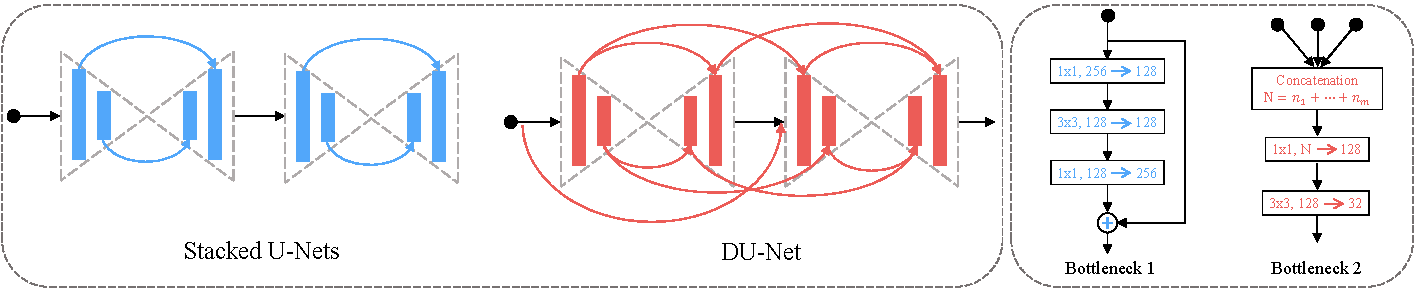
\includegraphics[width=1.0\linewidth]{figures/framework-cropped.pdf}
\caption{Illustration of stacked U-Nets and DU-Net. Stacked U-Nets has skip connections only within each U-Net. In contrast, DU-Net also connects blocks with the same semantic meanings across different U-Nets. The feature reuse could significantly reduce the size of bottleneck in each block, as shown in the right figure. Consequently, with the same number of U-Nets, DU-Net has only 30\% parameters of stacked U-Nets.}
\label{fig:framework}
\end{figure*}

% 
Our solution to those efficiency issues is threefold. {\bf First}, instead of connecting all stacked U-Nets, we only connect a U-Net to its $K$ successors. We name it as the $order$-$K$ connectivity, which aims to balance the fitting accuracy and parameter efficiency by cutting off long-distance connections. {\bf Second}, we employ a memory-efficient implementation in training. The key idea is to reuse a pre-allocated memory so all connected blocks could share the same memory. Compared with the naive implementation, this strategy makes it possible to train a very deep DU-Net (actually, $2\times$ deeper). {\bf Third}, to further improve the efficiency, we investigate an iterative design that may reduce the model size to one half. More specifically, the output of the first pass of the DU-Net is used as the input of the second pass, where detection or regression loss is applied as supervision. 

% %G%
% In view of deploying our approach on mobile devices, we further attempt to quantize weights, inputs, and gradients of DU-Net to low bit-width discrete values. This not only decreases the high precision operations but also shrinks the memory usage during training. By network quantization, the size of trained model can also be largely compressed.
% %G%
Besides shrinking the number of network parameters, we also study to further quantize each parameter. This motivates from the ubiquitous mobile applications. Although current mobile devices could carry models of dozens of MBs, deploying such networks requires high-end GPUs. However, quantized models could be accelerated by some specifically designed low-cost hardwares. Beyond only deploying models on mobile devices \cite{li2017deeprebirth}, training deep neural networks on distributed mobile devices emerges recently \cite{mcmahan2016communication}. To this end, we also try to quantize not only the model parameters but also its inputs (intermediate features) and gradients in training. This is the first attempt to investigate training landmark localizers using quantized inputs and gradients.


In summary, our key contributions are:
\begin{itemize}
    \item To the best of our knowledge, we are the first to propose quantized densely connected U-Nets for visual landmark localization, which largely improves the information flow and feature reuse at the semantic level.
    \item We propose the $order$-$K$ connectivity to balance accuracy and efficiency. It decreases the growth of model size from quadratic to linear by removing trivial connections. Experiments show it could reduce $\sim$70\% parameters of state-of-the-art landmark localizers.
    \item Very deep U-Nets can be trained using a memory-efficient implementation, where pre-allocated memory is reused by all connected blocks.
    \item We further investigate an iterative refinement that may cut down half of the model size, by forwarding DU-Net twice using either detection or regression supervision.
    %G%
    \item Different from previous efforts of quantizing only the model parameters, we are the first to quantize their inputs and gradients for better training efficiency on landmark localization tasks. By choosing appropriate quantization bit-widths for weights, inputs and gradients, quantized DU-Net achieves $\sim$75\% training memory saving with comparable performance. 
    %G%
    \item Exhaustive experiments are performed to validate DU-Net in different aspects. In both human pose estimation and face alignment, DU-Net demonstrates comparable localization accuracy and use $\sim$2\% model size compared with state-of-the-art methods.
\end{itemize}

% We are the first to deploy network quantization for better training efficiency on localization tasks. By choosing appropriate quantization bit-widths for weights, inputs and gradients, quantized DU-Net achieves at least 32$\times$ memory saving with comparable performance to the-state-of-art approaches. 


%The landmark localization such as human pose estimation \cite{toshev2014deeppose,newell2016stacked,wei2016convolutional}, facial landmark localization \cite{xiong2013supervised,zhang2014facial,sagonas2013300}, etc, plays an important role in the higher-level image understanding. The Convolutional Neural Networks (CNNs) have dominated this field, among which recent architecture of stacked hourglasses \cite{newell2016stacked}, a variant of the U-Net \cite{ronneberger2015unet}, becomes a standard solution. The skip connections between top-down and bottom-up blocks within a U-Net could preserve the spatial information and increase the gradient flow. With multiple U-Nets stacked together, the prediction could be refined stage by stage. However, the connections are only within each U-Net of the stacked hourglasses and no explicit connections exist between U-Nets, which may impede the information flow across them. And the blocks with the same semantics in different U-Nets cannot share features, leading to many redundant parameters. 

% Its success attributes to three key factors: repeated top-down, bottom-up inferences, intermediate supervisions and residual bottlenecks \cite{}. 

% The multiple stage top-down and bottom-up processing could better integrate both the local and global visual contexts into the final prediction. The intermediate supervision and residual bottlenecks, on the other hand, could alleviate the gradient vanish problem in deep networks.
%In this paper, we propose to densely connect stacked U-Nets by linking blocks with the same semantics in different U-Nets. We refer to this architecture as {\it Dense U-Nets}. The blocks in a U-Net could get direct inputs from its connected blocks in all preceding U-Nets, making the information flow more efficiently among the U-Nets. The feature reuse at each resolution could reduce the parameters in each block. The dense connectivity in our Dense U-Nets is different from that of DenseNet \cite{huang2016densely}. More specifically, layers only within each single block of the DenseNet are connected. In contrast, we connect blocks lying across the whole Dense U-Nets and connections of hierarchical blocks are mixed together. An illustration is given in Figure \ref{fig:framework}. We name it as the {\it global dense connectivity} to differentiate from the local one in the DenseNet.

% Besides, features in the Dense U-Nets are fused by the concatenation which could facilitate the information flow compared with the summation operation in the stacked hourglasses.

% Although the dense connectivity in our Dense U-Nets is similar with that of DenseNet \cite{}, 
% More recently, the DenseNet \cite{} achieves superior image classification performance over the ResNet \cite{} in terms of both the accuracy and model size, which benefits from the dense connections between layers. Its key insight is the feature reuse between layers of the same resolutions. The dense connectivity in the DenseNet, existing within one block, is local. By extending this principle, we propose a global dense connectivity, in contrast to the local connectivity in \cite{}, that blocks at the same locations of different U-Nets are connected. Hence, we refer to this architecture as {\it Dense U-Nets}. To our best knowledge, we are the first to generalize the local dense connectivity into the stacked U-Nets. 
% The global dense connectivity could make it easier to train much deeper stacked U-Nets.

% This motivates us to replace the residual modules  in the stacked hourglasses with the dense connected layers. However, this dense connectivity exists only locally within a contiguous  block in which all feature maps have the same spatial resolution. A U-Net, on the other hand, consists of a sequence of top-down and bottom-up blocks. A straight way is to turn each block into a dense block with multiple layers. However, this would sacrifice the spirit of stacked hourglasses that multiple stacked hourglasses outperform a single hourglass with multiple layers in each block.

% In order to integrate the structure of stacked U-Nets together with the idea of dense connectivity, we propose a global dense connectivity, in contrast to the local connectivity in \cite{}, that blocks at the same locations of different U-Nets are connected. Hence, we refer to this architecture as {\it Dense U-Nets}. The connected layers in the Dense U-Nets distribute along the whole network rather than in local continuous blocks. Compared with the local residual modules in the stacked hourglasses, the global dense connections could significantly facilitate the gradient to flow across stacked U-Nets.

%In practice, the Dense U-Nets have the efficiency problems of both parameter and training memory. First, suppose a Dense U-Nets contains $n$ U-Nets, there would be $O(n(n-1)/2)$ connections. Even though we use the dense bottleneck in Figure \ref{fig:framework}, the number of conv($1\times 1$) parameters still has the quadratic growth. Inspired from the Variable Order Markov (VOM) models \cite{begleiter2004prediction}, we propose the order-K connectivity that, instead of linking all the U-Nets, we connect only a fixed number of U-Nets. The goal is to use the minimum connections achieving the most obvious improvements. The multiple intermediate supervisions in the Dense U-Nets are good compensates for the order-K connectivity since they could provide additional gradients. The DenseNet does not have this advantage since it has only one supervision at the end.

% Furthermore, different from the DenseNet with only one supervision, the Dense U-Nets have multiple intermediate supervisions. The global dense connections plus the intermediate supervisions could bring faster convergence on the training set, but also gives rise to the concern of overfitting. Inspired from the Variable Order Markov (VOM) models \cite{}, we propose the order-K connectivity that, instead of linking all the U-Nets, we connect only a fixed number of U-Nets. The goal is to use the minimum connections achieving the most obvious improvement. Another advantage of order-K connectivity is that it has fewer parameters compared with the dense connectivity.

%Benefiting from the order-K connectivity, the Dense U-Nets could achieve comparable performance of stacked hourglasses with only one-third parameters. However, a naive implementation of the order-K connectivity could make the training very memory expensive. Therefore, we employ the memory efficient implementation \cite{pleiss2017memory}. The key idea is to share memories for time efficient operations such as concatenation and batch norm \cite{ioffe2015batch} within the connected layers. By pre-allocating a fixed memory, the later features produced by these operations would replace earlier features. So we need to re-compute those replaced features in the backward phase. The memory efficient implementation makes it possible to train Dense U-Nets two times deeper than the stacked hourglasses. 

%Furthermore, we also investigate to use the iterative refinement improving the parameter efficiency. Given a Dense U-Nets, we compare its performance with another Dense U-Nets with only half depth but an additional iteration. Besides, both detection and regression losses \cite{bulat2016human} were used in the landmark detection tasks, but there is no investigation yet about how they independently and collaboratively affect the prediction. We will give their detailed comparison in our experiments.

%In summary, the key contributions are:
%\begin{itemize}
%    \item To our best knowledge, we are the first to use the dense connectivity among the stacked U-Nets. The global dense connectivity in our Dense U-Nets is different from the local one in the DenseNet \cite{huang2016densely}.
%    \item We propose the order-K connectivity to make the Dense U-Nets parameter efficient. The order-K connectivity could decrease the growth of conv($1\times 1$) parameters from quadratic to linear. With comparable performance as the stacked hourglasses \cite{newell2016stacked}, it makes the Dense U-Nets require only one-third parameters. 
%    \item The memory efficient implementation of Dense U-Nets is provided to reduce its training memory usage. It makes it possible to train Dense U-Nets two times deeper than the stacked hourglasses.
%    \item We further explore using iterative refinement to improvement the parameter efficiency. At the same time, we investigate how different combinations of the detection and regression losses affect the performance.
%\end{itemize}

\begin{figure*}
\centering
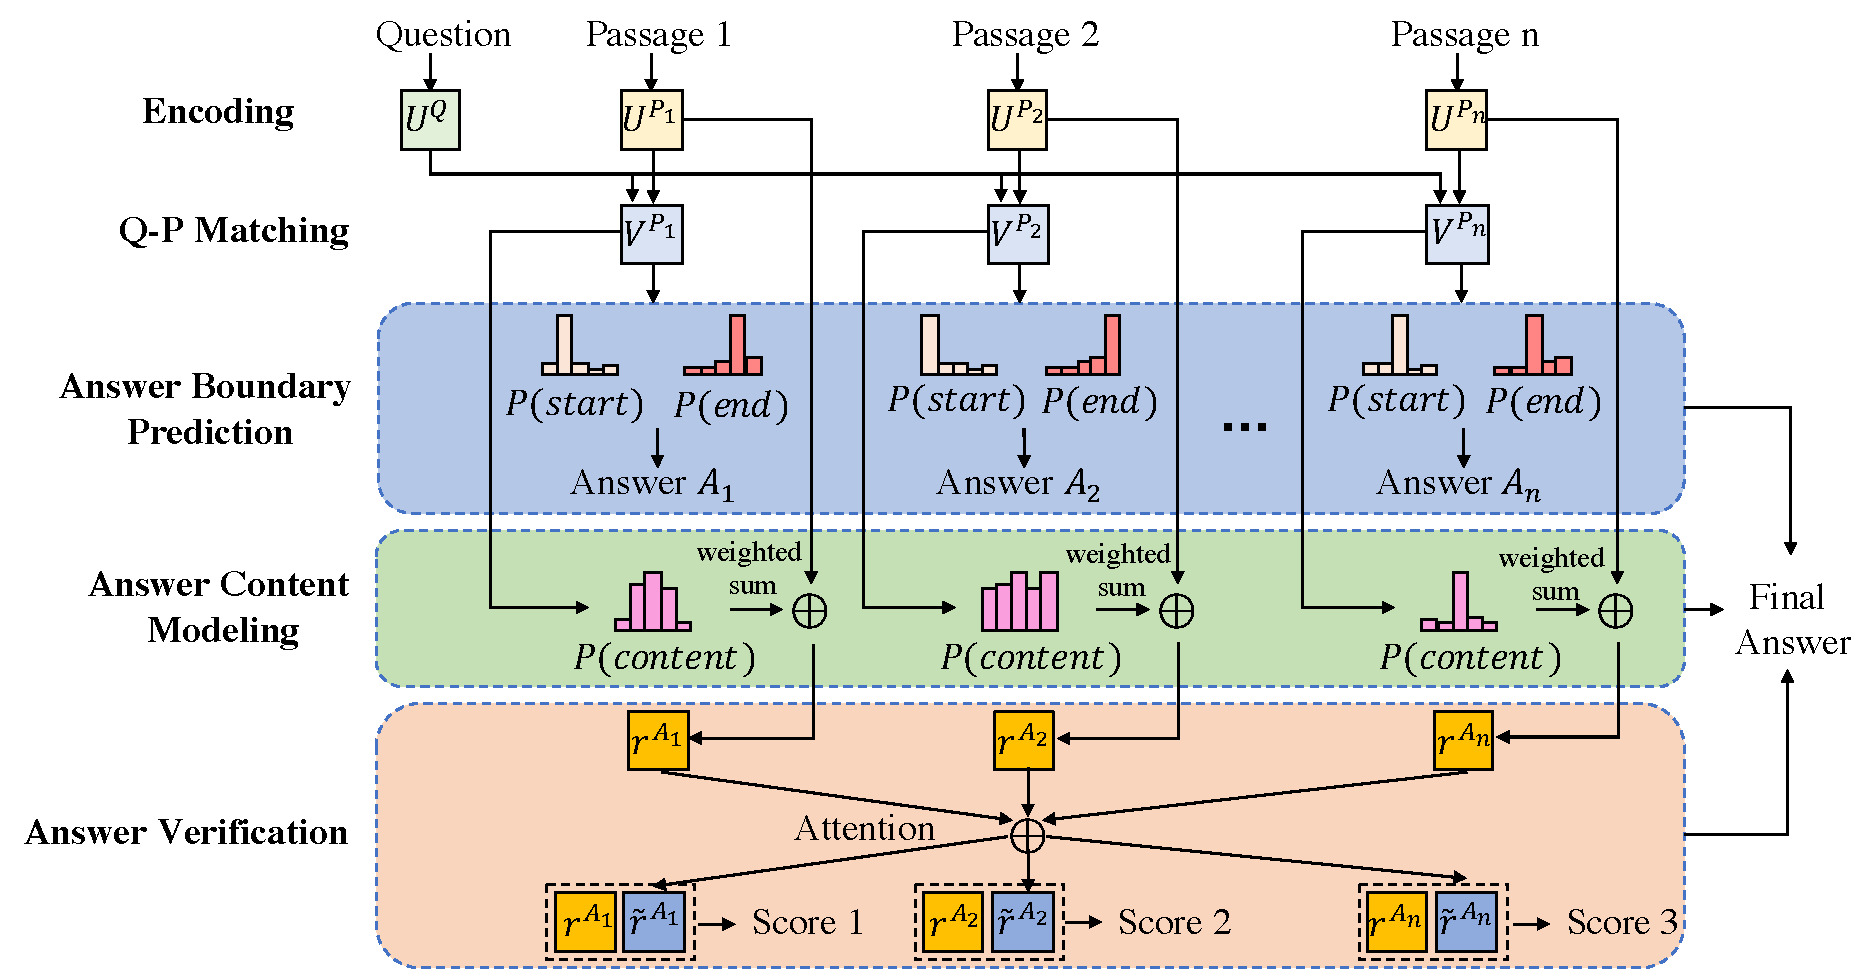
\includegraphics[width=0.85\textwidth]{architecture}
\caption{The overall architecture of our proposed network. The network
contains layers of symmetric convolution (encoder) and deconvolution (decoder).
Skip shortcuts are connected every a few (in our experiments, two) layers from
convolutional feature maps to their mirrored deconvolutional feature maps.
The response from a convolutional layer is directly propagated to the corresponding
mirrored deconvolutional layer, both forwardly and backwardly.}
\label{fig1}
\end{figure*}

\section{Very deep convolutional auto-encoder for image restoration}
\label{sec:main}

The proposed framework mainly contains a chain of convolutional layers and symmetric
deconvolutional layers, as shown in Figure \ref{fig1}. Skip connections are connected
symmetrically from convolutional layers to deconvolutional layers. We term our method
``RED-Net''---very deep Residual Encoder-Decoder Networks.


\subsection{Architecture}

The framework is fully convolutional (and deconvolutional.  Deconvolution is essentially unsampling convolution). Rectification layers are added
after each convolution and deconvolution. For low-level image restoration problems, we
use neither pooling nor unpooling in the network as usually pooling discards useful image
details that are essential for these tasks. It is worth mentioning that since the convolutional
and deconvolutional layers are symmetric, the network is essentially pixel-wise prediction,
thus the size of input image can be arbitrary. The input and output of the network are images
of the same size $w\times h\times c$, where $w$, $h$ and $c$ are width, height and number of channels.

Our main idea is that the convolutional layers act as a feature extractor, which preserve the
primary components of objects in the image and meanwhile eliminating the corruptions.
After forwarding through the convolutional layers, the corrupted input  image is converted into
a ``clean" one. The subtle details of the image contents may be lost during this process.
The deconvolutional layers are then combined to recover the details of image contents.
The output of the deconvolutional layers is the recovered clean version of the input image.
Moreover, we add skip connections  from a convolutional layer to its corresponding
mirrored deconvolutional layer. The passed convolutional feature maps are summed to the
deconvolutional feature maps element-wise, and passed to the next layer after rectification.
Deriving from the above architecture, we have used two networksvin our experiments, which are of 20 layers
 and 30 layers
respectively, for image denoising, image super-resolution, JPEG deblocking and image inpainting.



\subsection{Deconvolution decoder}

Architectures combining layers of convolution and deconvolution~\cite{DBLP:conf/iccv/NohHH15,
hong2015decoupled} have been proposed for semantic segmentation recently. In contrast to
convolutional layers, in which multiple input activations within a filter window are fused
to output a single activation, deconvolutional layers associate a single input activation with
multiple outputs. Deconvolution is usually used as {\em learnable up-sampling layers}.

 In our network,
the convolutional layers successively down-sample the input image content into a  small
size abstraction. Deconvolutional layers then up-sample the abstraction back into its original resolution.

Besides the use of skip connections, a main difference between our model and
~\cite{DBLP:conf/iccv/NohHH15,hong2015decoupled} is that our network is fully convolutional and
deconvolutional, i.e., without pooling and un-pooling. The reason is that for low-level image restoration,
the aim is to eliminate low level corruption while preserving image details instead of learning
image abstractions. Different from high-level applications such as segmentation or recognition,
pooling typically eliminates the abundant image details and can deteriorate restoration performance.



One can simply replace deconvolution with convolution, which results in an architecture that is
very similar to recently proposed very deep fully convolutional neural networks
~\cite{DBLP:conf/cvpr/LongSD15,DBLP:journals/pami/DongLHT16}. However, there exist essential
differences between a fully convolution model and our model. Take image denoising as an example.
We compare the 5-layer and 10-layer fully convolutional network with our network
(combining convolution and deconvolution, but without skip connection). For fully convolutional
networks, we use padding or up-sampling the input to make the input and output be of the same size.
For our network, the first 5 layers are convolutional and the second 5 layers are deconvolutional.
All the other parameters for training are identical, i.e., trained with SGD and learning rate of
$10^{-6}$, noise level $\sigma=70$. The Peak Signal-to-Noise Ratio (PSNR) on the validation set
is reported, which shows that using deconvolution works better than the fully convolutional
counterpart, as shown in Figure \ref{fig2}.


Furthermore, in Figure \ref{fig3}, we visualize some results that are outputs of layer 2, 5, 8 and 10
from the 10-layer fully convolutional network and ours. In the fully convolution case, the noise
is eliminated step by step, i.e., the noise level is reduced after each layer. During this process,
the details of the image content may be lost. Nevertheless, in our network, convolution  preserves
the primary image content. Then deconvolution is used to compensate the details.


\begin{figure}[htb!]
\centering
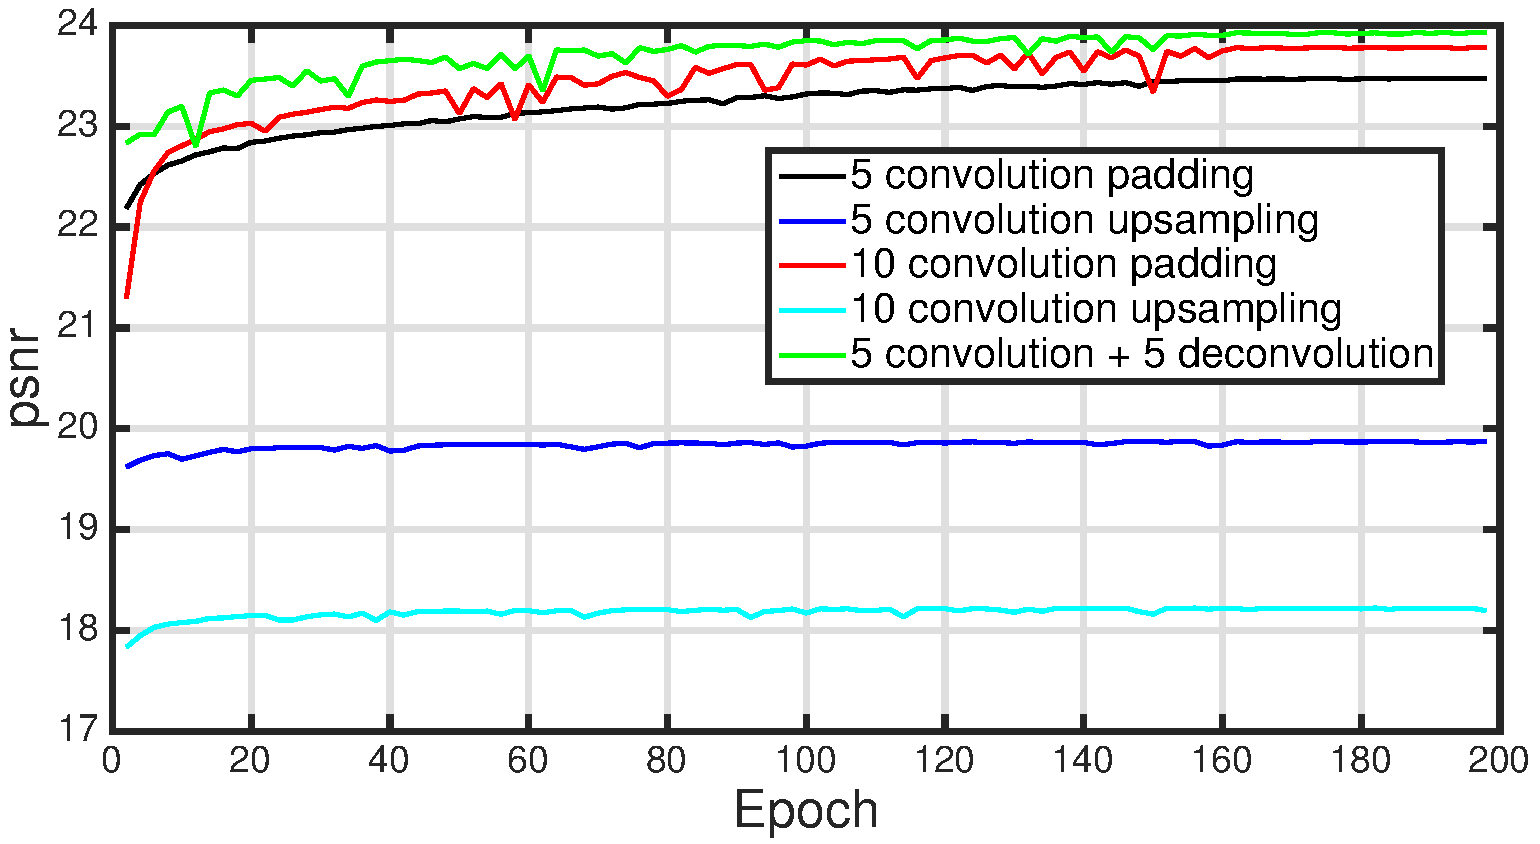
\includegraphics[width=0.48\textwidth]{conv-vs-decv}
\caption{ PSNR  values  on the validation set during training. Our model  exhibits better PSNR
than the compared ones upon convergence.}
\label{fig2}
\end{figure}



\begin{figure}[htb!]
\centering
\subfigure[]{ 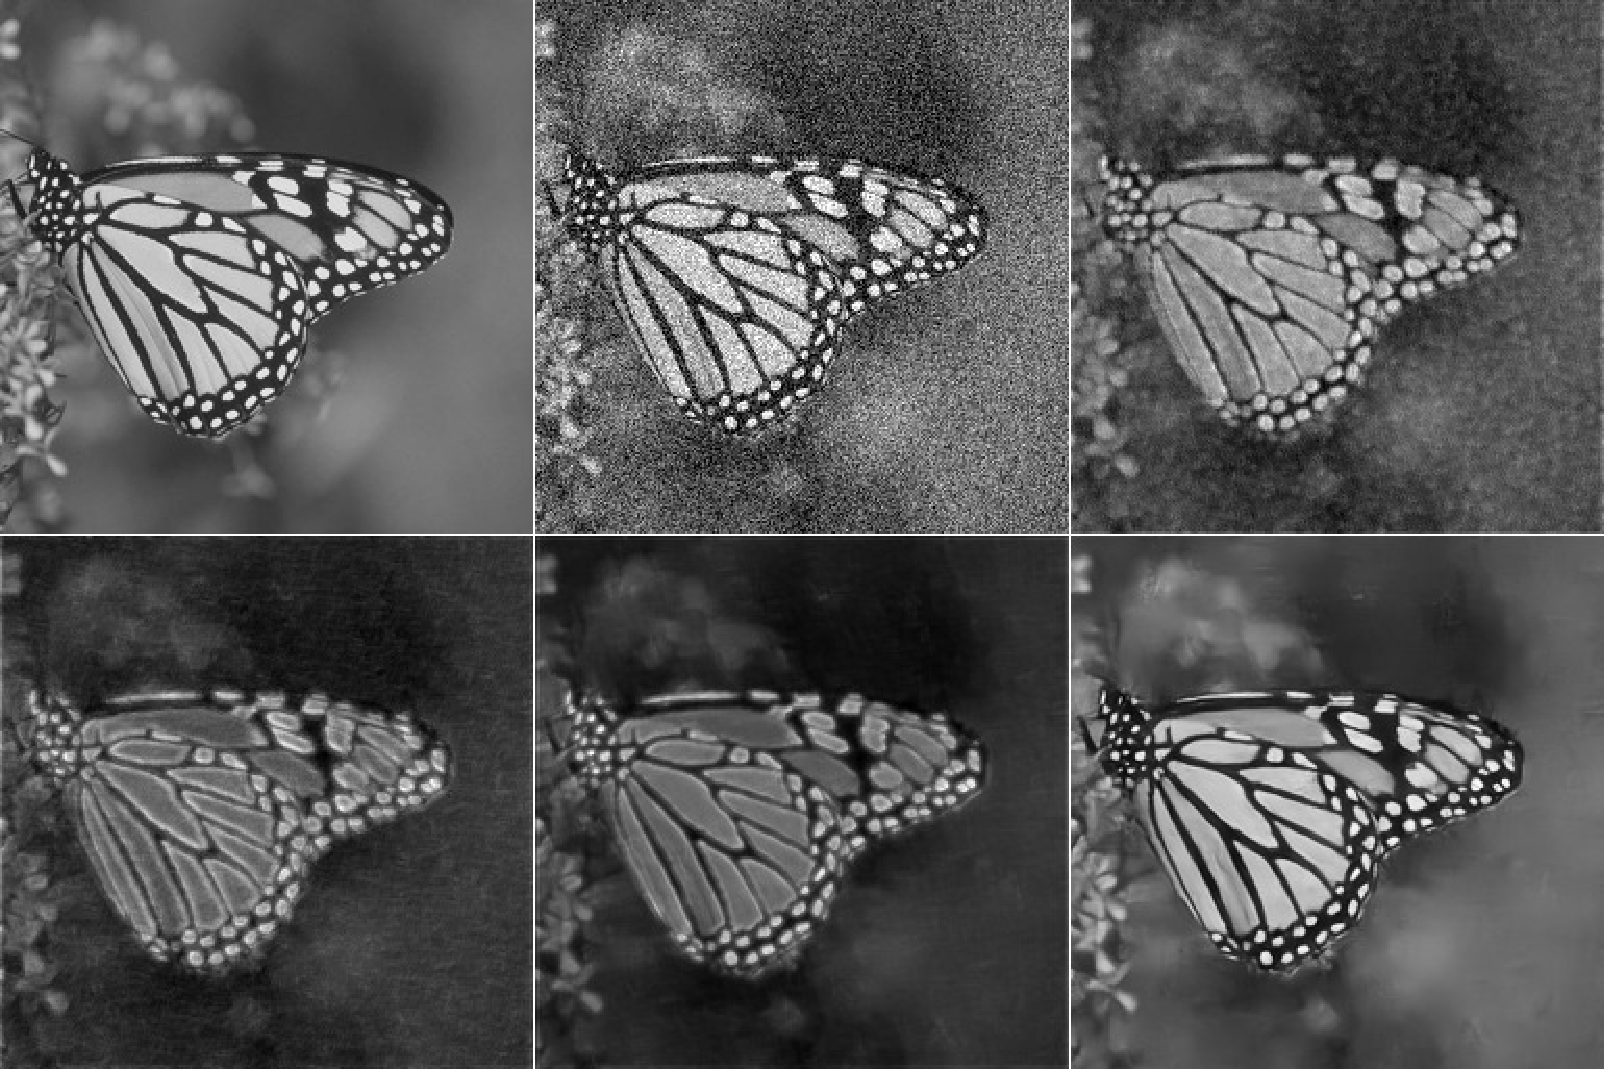
\includegraphics[width=0.48\textwidth]{show-denoising-conv} }
\subfigure[]{ 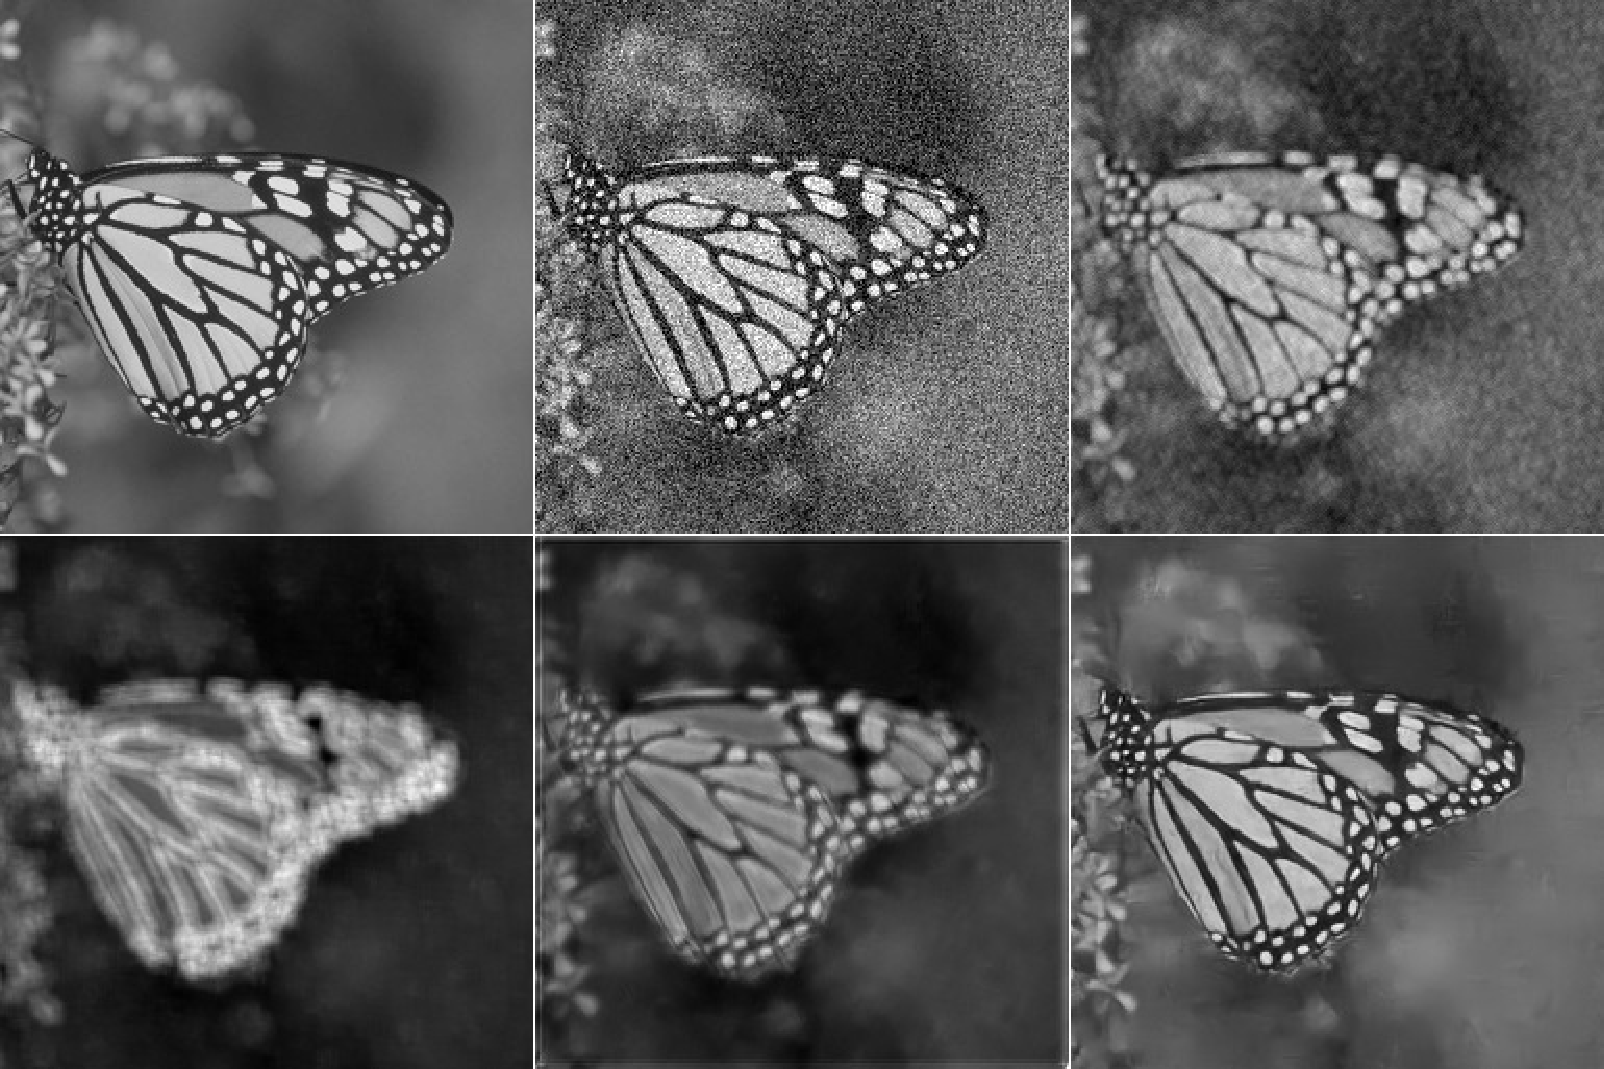
\includegraphics[width=0.48\textwidth]{show-denoising-decv} }
\caption{ (a) Visualization of the 10-layer fully convolutional network. The images from
top-left to bottom-right are: clean image, noisy image, output of conv-2, output of conv-5,
output of conv-8 and output of conv-10, where ``conv-$i$" stands for the $i$-th convolutional layer;
(b) Visualization of the 10-layer convolutional and deconvolutional network. The images from
top-left to bottom-right are: clean image, noisy image, output of conv-2, output of conv-5,
output of deconv-3 and output of deconv-5, where ``deconv-$i$" stands for the $i$-th deconvolutional layer.}
\label{fig3}
\end{figure}




\subsection{Skip connections}

An intuitive question is that, is a network with deconvolution able to recover image details from
the image abstraction only? We find that in shallow networks with only a few layers
of convolution layers, deconvolution is able to recover the details. However, when the
network goes deeper or using operations such as max pooling, even with deconvolution layers, it does not work
that well, possibly because too much details are already lost in the convolution and pooling.


The second question is that, when our network goes deeper, does it achieve performance gain?
We observe that deeper networks in image restoration tasks tend to easily suffer from
performance degradation. The reason may be two folds. First of all, with more layers of
convolution, a significant amount of image details could be lost or corrupted. Given only the image abstraction,
recovering its details is an under-determined problem. Secondly, in terms of optimization,
deep networks often suffer from gradients vanishing and become much harder to train---a problem
that is well addressed in the literature of neural networks.


To address the above two problems, inspired by highway networks \cite{DBLP:journals/corr/SrivastavaGS15}
and deep residual networks \cite{DBLP:journals/corr/HeZRS15}, we add skip connections between
two corresponding convolutional and deconvolutional layers as shown in Figure \ref{fig1}.
A building block is shown in Figure \ref{fig4}. There are two reasons for using such connections.
First, when the network goes deeper, as mentioned above, image details can be lost, making deconvolution
weaker in recovering them. However, the feature maps passed by skip connections carry much image detail,
which helps deconvolution to recover an improved clean version of the image. Second, the skip connections also achieve
benefits on back-propagating the gradient to bottom layers, which makes training deeper network much
easier as observed in \cite{DBLP:journals/corr/SrivastavaGS15} and \cite{DBLP:journals/corr/HeZRS15}.

Note that our skip layer connections are very different from the ones proposed in
\cite{DBLP:journals/corr/SrivastavaGS15} and \cite{DBLP:journals/corr/HeZRS15}, where the only concern
is on the optimization side. In our case, we want to pass information of the convolutional feature maps
to the corresponding deconvolutional layers. The very deep highway networks
\cite{DBLP:journals/corr/SrivastavaGS15} are essentially feedforward long short-term memory (LSTMs)
with forget gates, and the CNN layers of deep residual network \cite{DBLP:journals/corr/HeZRS15}
are feedforward LSTMs without gates. Note that our networks are in general not in the format of
standard feedforward LSTMs.

\begin{figure}[htb!]
\centering
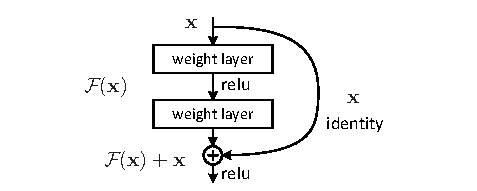
\includegraphics[width=0.48\textwidth]{block}
\caption{An example of a building block in the proposed framework. The rectangle in solid and
dotted lines denote convolution and deconvolution respectively. $\oplus$ denotes element-wise sum of feature maps.}
\label{fig4}
\end{figure}

Instead of directly learning the mappings from the input $X$ to the output $Y$, we would like the network
to fit the residual~\cite{DBLP:journals/corr/HeZRS15} of the problem, which is denoted as $\mathcal{F}(X)=Y-X$.
Such a learning strategy is applied to inner blocks of the encoding-decoding network to make training more
effective. Skip connections are passed every two convolutional layers to their mirrored deconvolutional
layers. Other configurations are possible and our experiments show that this configuration already works
very well. Using such shortcuts makes the network easier to be trained and gains restoration performance
by increasing the network depth.




\subsection{Training}

In general, there are three types of layers in our network: convolution, deconvolution
and element-wise sum. Each layer is followed by a Rectified Linear Unit (ReLU)
~\cite{DBLP:conf/icml/NairH10}. Let $X$ be the input, the convolutional and
deconvolutional layers are expressed as:
\begin{equation}
F(X) = \max(0,W_k * X + B_k),
\end{equation}
where $W_k$ and $B_k$ represent the filters and biases, and $*$ denotes either
convolution or deconvolution operation for the convenience of formulation.
For element-wise sum layer, the output is the element-wise sum of two inputs
of the same size, followed by the ReLU activation:
\begin{equation}
F(X_1,X_2) = \max(0, X_1 + X_2)
\end{equation}

Learning the end-to-end mapping from corrupted images to clean images needs to
estimate the weights $\Theta$ represented by the convolutional and deconvolutional
kernels. Specifically, given a collection of $N$ training sample pairs $\{X^i,Y^i\}$,
where $X^i$ is a noisy image and $Y^i$ is the clean version as the groundtruth.
We minimize the following Mean Squared Error (MSE):
\begin{equation}
  \mathcal{L}(\Theta) = \frac{1}{N}\sum_{i=1}^{N}\|\mathcal{F}(X^i;\Theta)-Y^i\|_F^2.
\label{eq1}
\end{equation}

Traditionally, a  network can learn the mapping from the corrupted image to the clean version
directly. However, our network learns for the additive corruption from the input since there
is a skip connection between the input and the output of the network.
%
%
%
We found that optimizing for the corruption converges better than
optimizing for the clean image. In the extreme case, if the input is a clean image, it would be easier
to push the network to be zero mapping (learning the corruption) than to fit an identity
mapping (learning the clean image) with a stack of nonlinear layers.

We implement and train our network using Caffe~\cite{jia2014caffe}. Empirically, we find
that using Adam~\cite{DBLP:journals/corr/KingmaB14} with base learning rate of $10^{-4}$ for
training converges faster than traditional stochastic gradient descent (SGD). The base
learning rate for all layers are the same, different from ~\cite{DBLP:journals/pami/DongLHT16,
DBLP:conf/nips/JainS08}, in which a smaller learning rate is set for the last layer.
This  is not necessary in our network. Specifically, gradients with respect to the
parameters of $i$th layer is firstly computed as:
\begin{equation}
g = \nabla_{\theta_i}\mathcal{L}(\theta_i).
\end{equation}
Then, the two momentum vectors are computed as:
\begin{equation}
m = \beta_1m + (1 - \beta_1)g,\quad v = \beta_2v + (1-\beta_2)g^2.
\end{equation}
The update rule is:
\begin{equation}
\alpha = \alpha\sqrt{1-\beta_2^t}/(1-\beta_1^t), \quad \theta_i=\theta_i-\alpha m/(\sqrt{v}+\epsilon).
\end{equation}
$\beta_1$, $\beta_2$ and $\epsilon$ are set as the recommended values in~\cite{DBLP:journals/corr/KingmaB14}.

300 images from the Berkeley Segmentation Dataset (BSD)~\cite{MartinFTM01} are used to
generate image patches as the training set for each image restoration task.
%
%
%




\subsection{Testing}

Although trained on local patches, our network can perform restoration on images of arbitrary sizes.
Given a testing image, one can simply go forward through the network, which is already able to
 outperform existing methods. To achieve even better results, we propose
to process a corrupted image on multiple orientations. Different from segmentation, the
filter kernels in our network only eliminate the corruptions, which is usually not sensitive
to the orientation of image contents in low level restoration tasks. Therefore, we can rotate
and mirror flip the kernels and perform forward multiple times, and then average the output to
achieve an ensemble of multiple tests. We see that this can lead to slightly better performance.


% !TeX root=../journalDeepMedic.tex


%%%%%%%%%%%%%%%%%%%%%%%%%%%%%%%%%%%%%%%%%%%%%%%%%%%%%%%%%%%%%%
%%%%%%%%%%% Validation of the Architecture %%%%%%%%%%%%%%%%%%%
%%%%%%%%%%%%%%%%%%%%%%%%%%%%%%%%%%%%%%%%%%%%%%%%%%%%%%%%%%%%%%

\section{Analysis of Network Architecture}
\label{sec:vaOfNetArch}

In this section we present a series of experiments in order to analyze the impact of each of the main contributions and to justify the choices made in the design of the proposed 11-layers, multi-scale 3D CNN architecture, referred to as the \textit{DeepMedic}. Starting from the CNN baseline as discussed in Sec.~\ref{subsec:theBaseline}, we first explore the benefit of our proposed dense training scheme (cf. Sec.~\ref{subsec:denseTraining}), then investigate the use of deeper models (cf. Sec.~\ref{subsec:buildingADeeperNetwork}) and then evaluate the influence of the multi-scale dual pathway (cf. Sec.~\ref{subsec:multiscaleCnn}). Finally, we compare our method with corresponding 2D variants to assess the benefit of processing 3D context.

\subsection{Experimental Setting}
\label{subsec:experimentSetting}

The following experiments are conducted using the TBI dataset with 61 multi-channel MRIs which is described in more detail later in Sec.~\ref{subsec:evalTbi}. Here, the images are randomly split into a validation and training set, with 15 and 46 images each. The same sets are used in all analyses. To monitor the progress of segmentation accuracy during training, we extract 10k random patches at regular intervals, with equal numbers extracted from each of the validation images. The patches are uniformly sampled from the brain region in order to approximate the true distribution of lesions and healthy tissue. Full segmentation of the validation datasets is performed every five epochs and the mean Dice similarity coefficient (DSC) is determined. Details on the configuration of the networks are provided in \ref{app:detailsConfig}.

\subsection{Effect of Dense Training on Image Segments}
\label{subsec:valDenseTraining}

\begin{figure}[!h]
\centering
\begin{subfigure}[b]{1.0\textwidth}
\centering
	%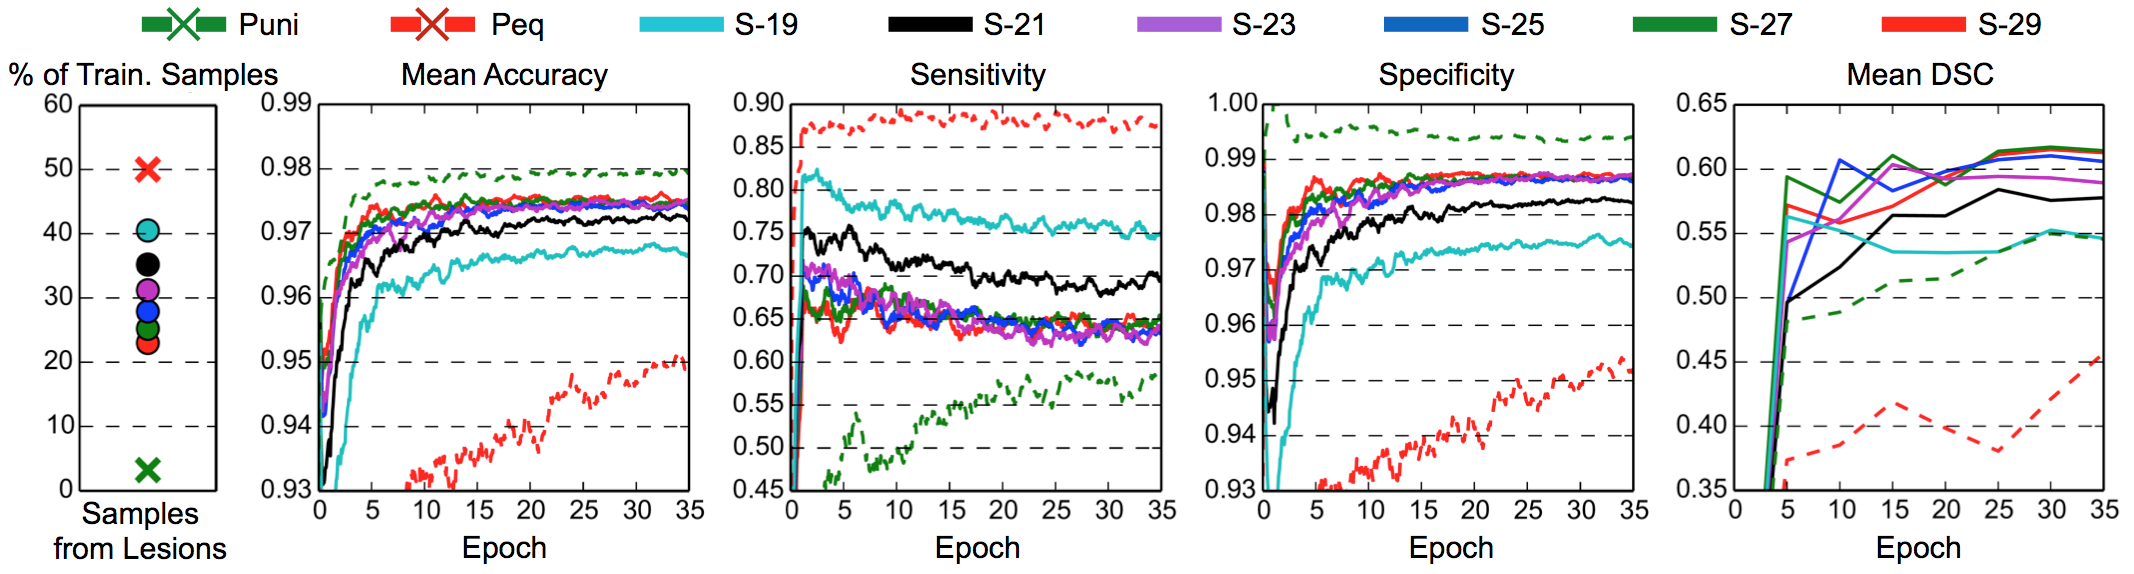
\includegraphics[clip=true, trim=10pt 270pt 30pt 210pt, width=1.0\textwidth]{figures/validationOfArchitecture/denseTraining/denseFigureToPlace.pdf}
	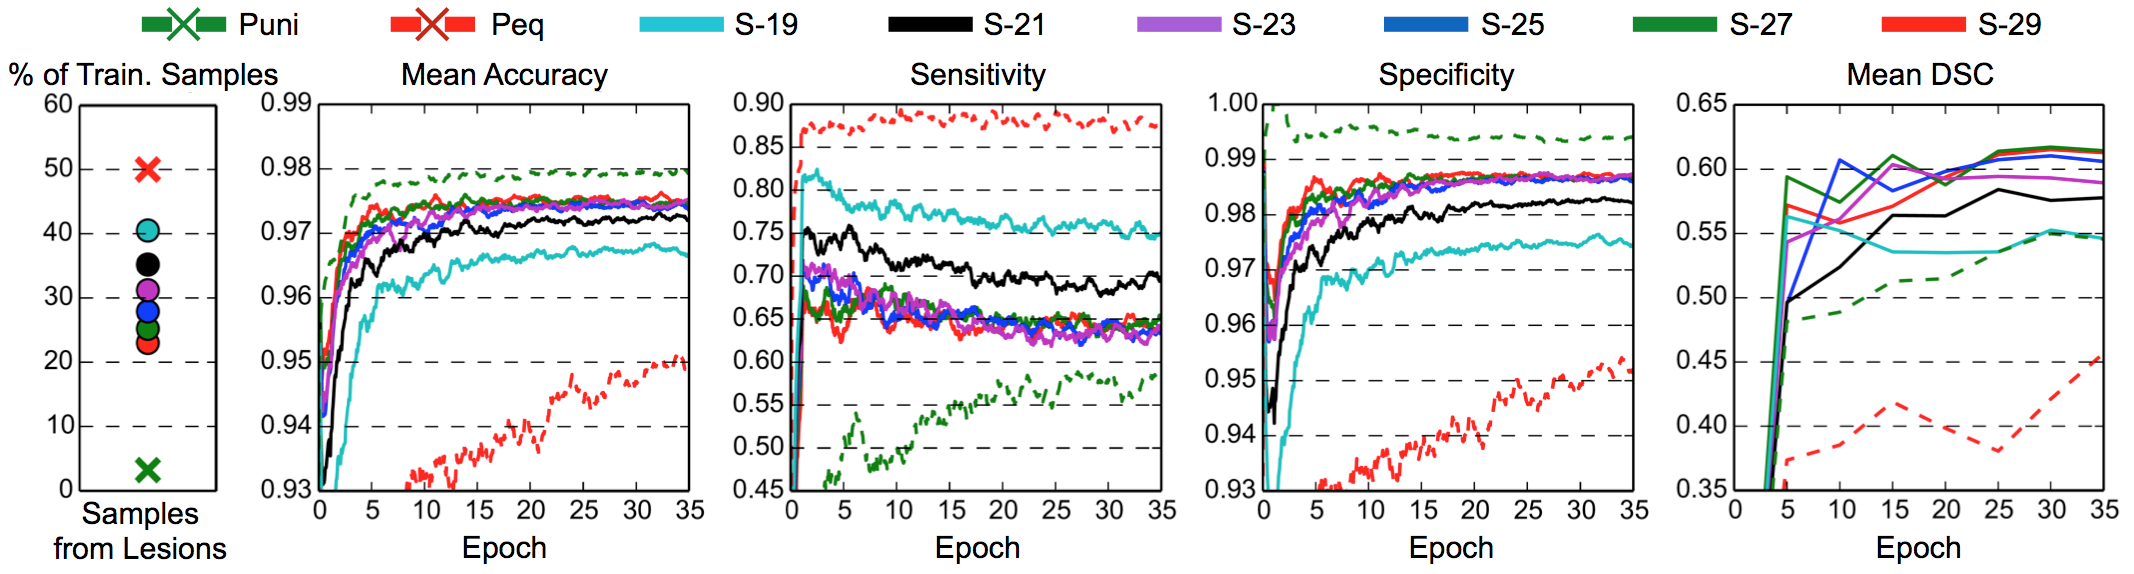
\includegraphics[clip=true, trim=0pt 0pt 0pt 0pt, width=1.0\textwidth]{figures/validationOfArchitecture/denseTraining/denseFigureToPlace.png}
\end{subfigure}
\caption{Comparison of the commonly used methods for training on patches uniformly sampled from the brain region (P$_\text{uni}$) and equally sampled from lesion and background (P$_\text{eq}$) against our proposed scheme (S-${d}$) on cubic segments of side length $d$, also equally sampled from lesion and background. We varied $d$ to observe its effect. From left to right: percentage of training samples extracted from the lesion class, mean accuracy, sensitivity, specificity calculated on uniformly sampled validation patches and, finally, the mean DSC of the segmentation of the validation datasets. The progress throughout training is plotted. Because lesions are small, P$_\text{uni}$ achieves very high voxel-wise accuracy by being very specific but not sensitive, with the opposite being the case for P$_\text{eq}$. Our method achieves an effective balance between the two, resulting in better segmentation as reflected by higher DSC.}
\label{fig:denseTrainingExperiment}
\end{figure}
%\vspace{-1pt} %takes away some white space before figure

We compare our proposed dense training method with two other commonly used training schemes on the 5-layers baseline CNN (see Fig.~\ref{fig:cnnBaseline}). The first common scheme trains on $17^3$ patches extracted uniformly from the brain region, and the second scheme samples patches equally from the lesion and background class. We refer to these schemes as P$_\text{uni}$ and P$_\text{eq}$. The results shown in Fig.~\ref{fig:denseTrainingExperiment} show a correlation of sensitivity and specificity with the percentage of training samples that come from the lesion class. P$_\text{eq}$ performs poorly because of over-segmentation (high sensitivity, low specificity). P$_\text{uni}$ has better classification on the background class (high specificity), which leads to high mean voxel-wise accuracy since the majority corresponds to background, but not particularly high DSC scores due to under-segmentation (low sensitivity).

To evaluate our dense training scheme, we train multiple models with varying sized image segments, equally sampled from lesions and background. The tested sizes of the segments go from $19^3$ upwards to $29^3$. The models are referred to as \quot{S-$d$}, where $d$ is the side length of the cubic segments. For fair comparison, the batch sizes in all the experiments are adjusted to have a similar memory footprint and lead to similar training times as compared to training on P$_{uni}$ and P$_{eq}$\footnote{Dense training on a whole volume was inapplicable in these experimental settings due to memory limitations but was previously shown to give similar results as training on uniformly sampled patches (\cite{Long2014}).}. We observe a great performance increase for model S-${19}$ over P$_\text{eq}$. We account this partly to the efficient increase of the effective batch size ($B \cdot V$ in Eq.~(\ref{eq:costDense})), but also to the altered distribution of training samples. As we increase the size of the training segments further, we quickly reach a balance between the sensitivity of P$_{eq}$ and the specificity of P$_{uni}$, which results in improved segmentation as expressed by the DSC.

The segment size is a hyper-parameter in our model. We observe that the increase in performance with increasing segment size quickly levels off, and similar performance is obtained for a wide range of segment sizes, which allows for easy configuration. For the remaining experiments, all models were trained on segments of size $25^3$.


\subsection{Effect of Deeper Networks}
\label{subsec:valDeeper}

\begin{figure}[!h]
\centering
\begin{subfigure}[b]{0.5\textwidth}
\centering
	%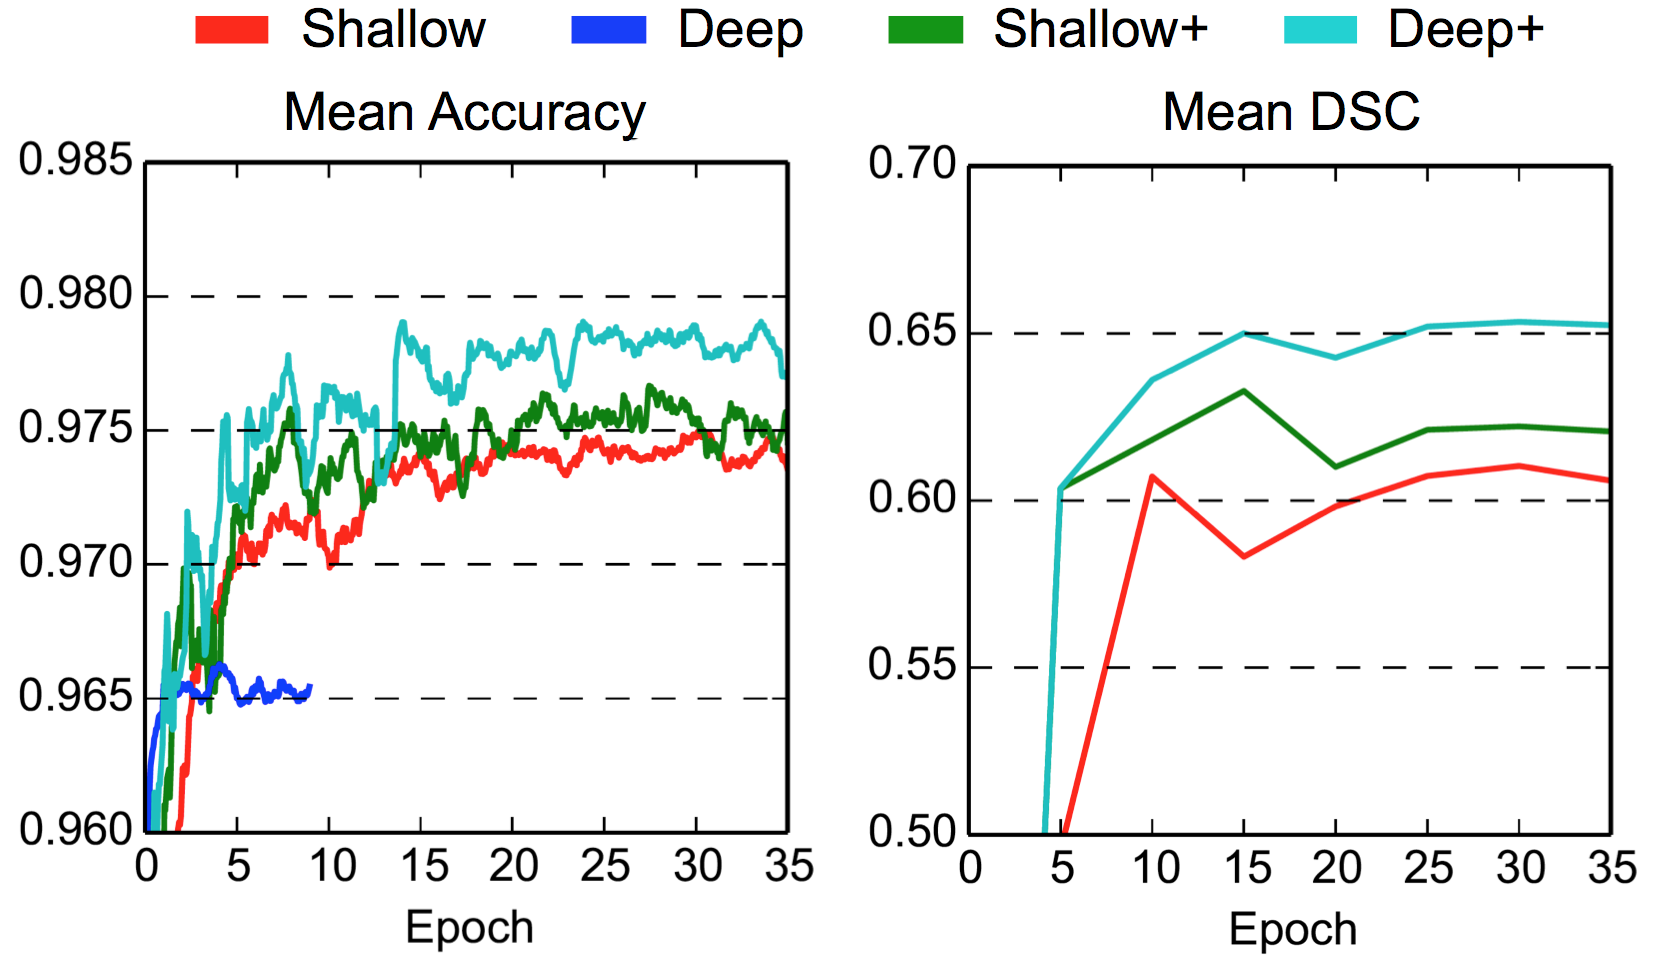
\includegraphics[clip=true, trim=50pt 30pt 140pt 250pt, width=1.0\textwidth]{figures/validationOfArchitecture/deepProblems/deepFigureToPut.pdf}
	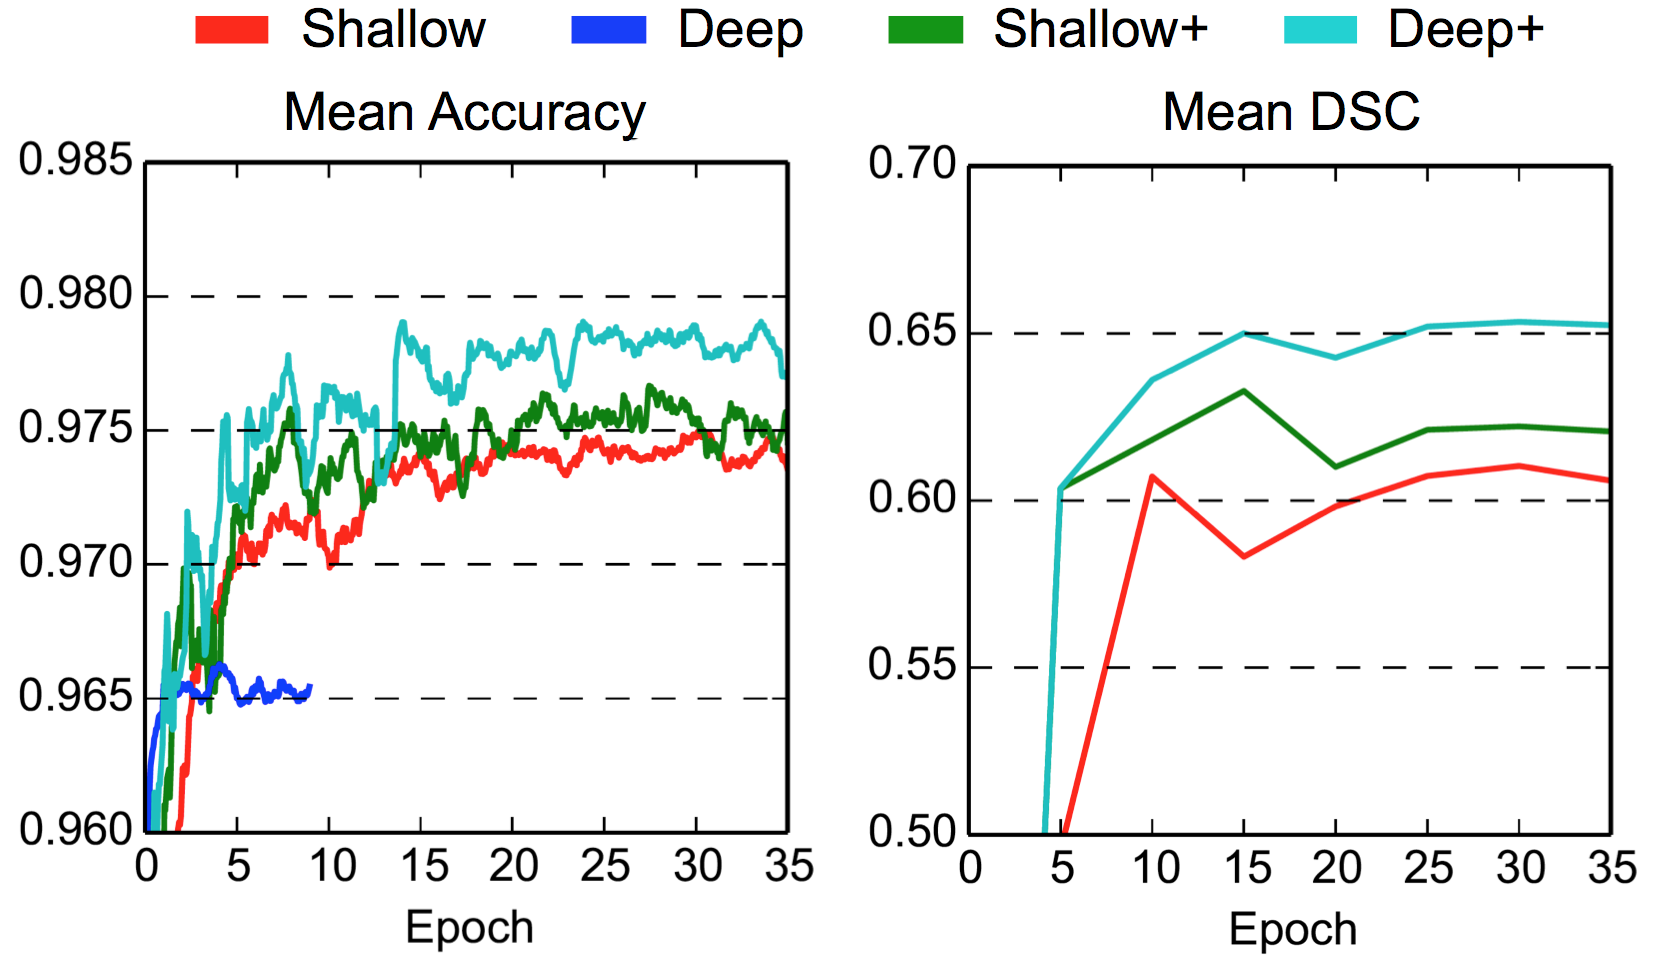
\includegraphics[clip=true, trim=0pt 0pt 0pt 0pt, width=1.0\textwidth]{figures/validationOfArchitecture/deepProblems/deepFigureToPut.png}
\end{subfigure}
\caption{Mean accuracy over validation samples and DSC for the segmentations of the validation images, as obtained from the \quot{Shallow} baseline and \quot{Deep} variant with smaller kernels. Training of the plain deeper model fails (cf. Sec.~\ref{subsec:valDeeper}). This is overcome by adopting the initialization scheme of (\cite{he2015delving}), which further combined with Batch Normalization leads to the enhanced (\texttt{+}) variants. Deep\texttt{+} performs significantly better than Shallow\texttt{+} with similar computation time, thanks to the use of small kernels.
}
\label{fig:deepProblems}
\end{figure}
%\vspace{-1pt} %takes away some white space before figure

The 5-layers baseline CNN (Fig.~\ref{fig:cnnBaseline}), here referred to as the \quot{Shallow} model, is extended to 9-layers by replacing each convolutional layer that uses $5^3$ kernels with two layers that use $3^3$ kernels (Fig.~\ref{fig:deeper3x3}). This model is referred to as \quot{Deep}. Training the latter, however, utterly fails with the model making only predictions corresponding to the background class. This problem is related to the challenge of preserving the signal as it propagates through deep networks and its variance gets multiplied with the variance of the weights, as previously discussed in Sec.~\ref{subsec:buildingADeeperNetwork}. One of the causes is that the weights of both models have been initialized with the commonly used scheme of sampling from the normal distribution $\mathcal{N}(0,0.01)$ (cf. \cite{Krizhevsky2012}). In comparison, the initialization scheme by \cite{he2015delving}, derived for preserving the signal in the initial stage of training, results in higher values and overcomes this problem. Further preservation of the signal is obtained by employing Batch Normalization. This results in an enhanced 9-layers model which we refer to as \quot{Deep\texttt{+}}, and using the same enhancements on the Shallow model yields \quot{Shallow\texttt{+}}. The significant performance improvement of Deep\texttt{+} over Shallow\texttt{+}, as shown in Fig.~\ref{fig:deepProblems}, is the result of the greater representational power of the deeper network. The two models need similar computational times, which highlights the benefits of utilizing small kernels in the design of 3D CNNs. Although the deeper model requires more sequential (layer by layer) computations on the GPU, those are faster due to the smaller kernel size.

\subsection{Effect of the Multi-Scale Dual Pathway}
\label{subsec:valMultiscale}

\begin{figure}[!h]
\centering
\begin{subfigure}[b]{0.5\textwidth}
\centering
	%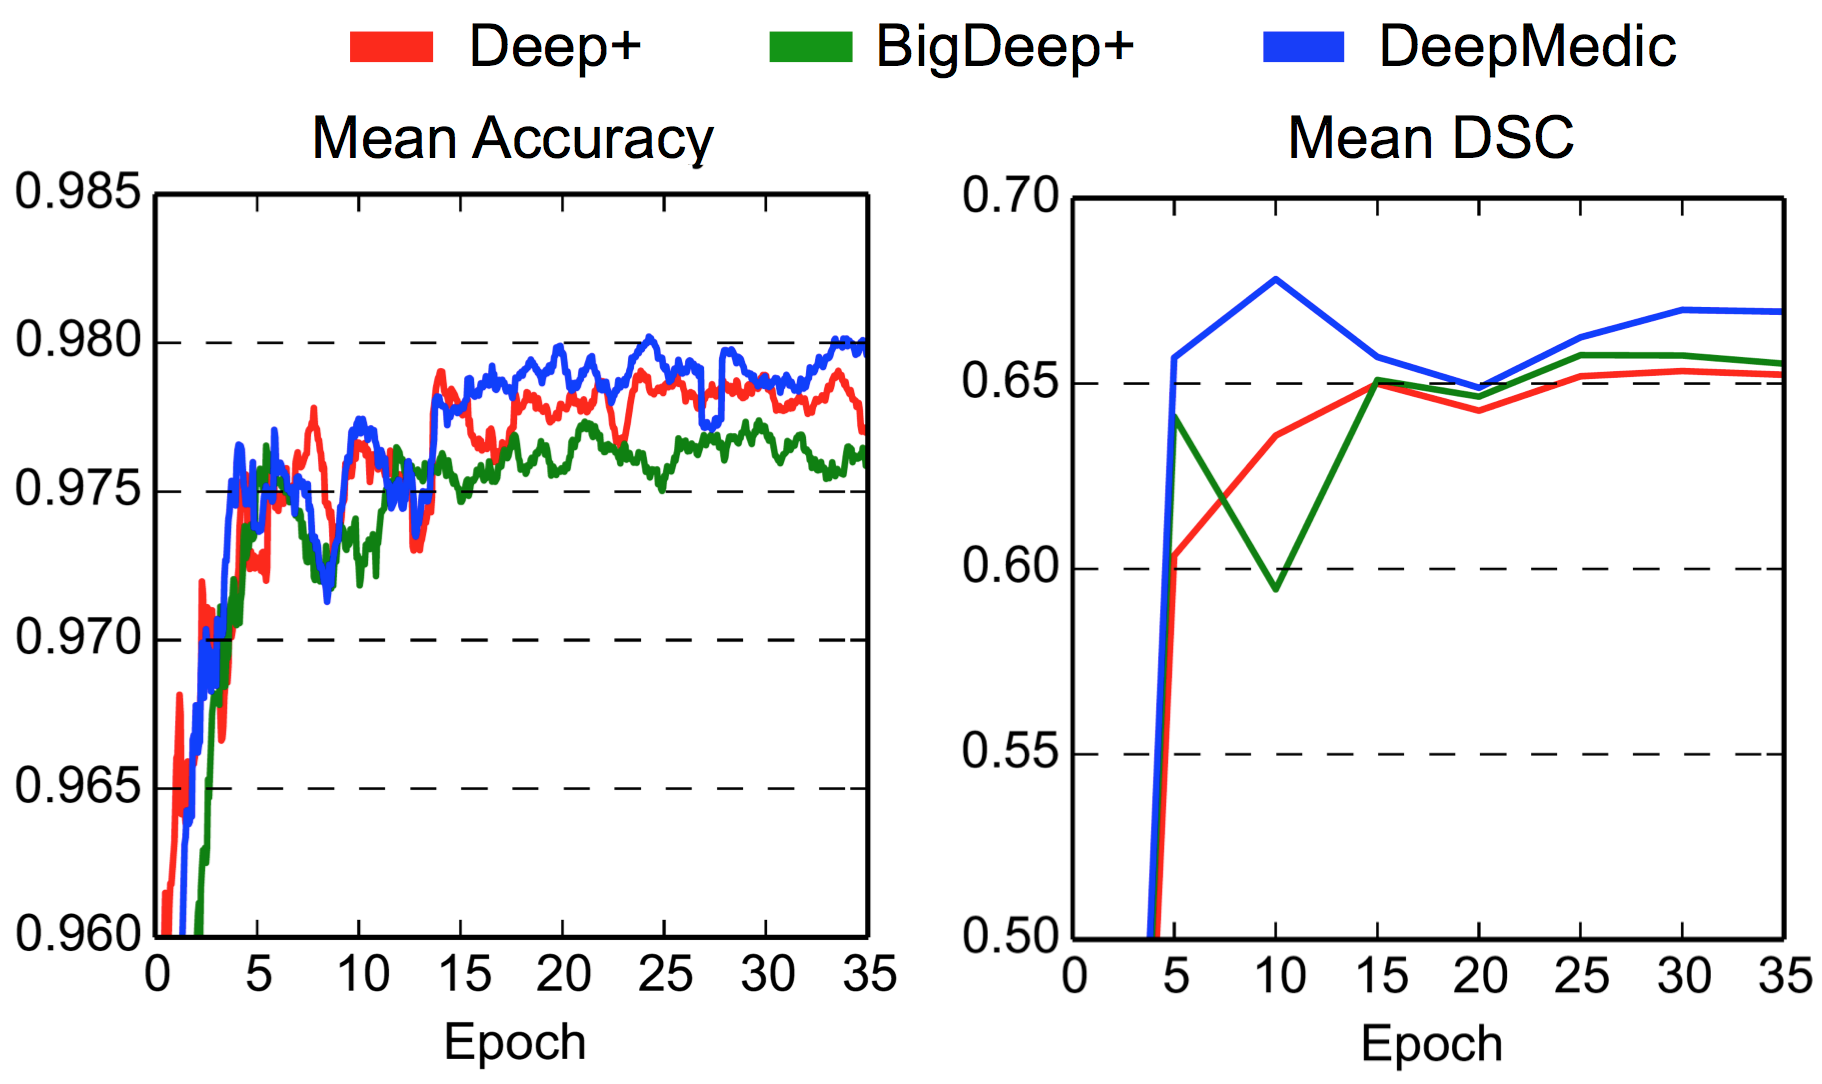
\includegraphics[clip=true, trim=50pt 30pt 140pt 250pt, width=1.0\textwidth]{figures/validationOfArchitecture/multiscale/figureToPut.pdf}
	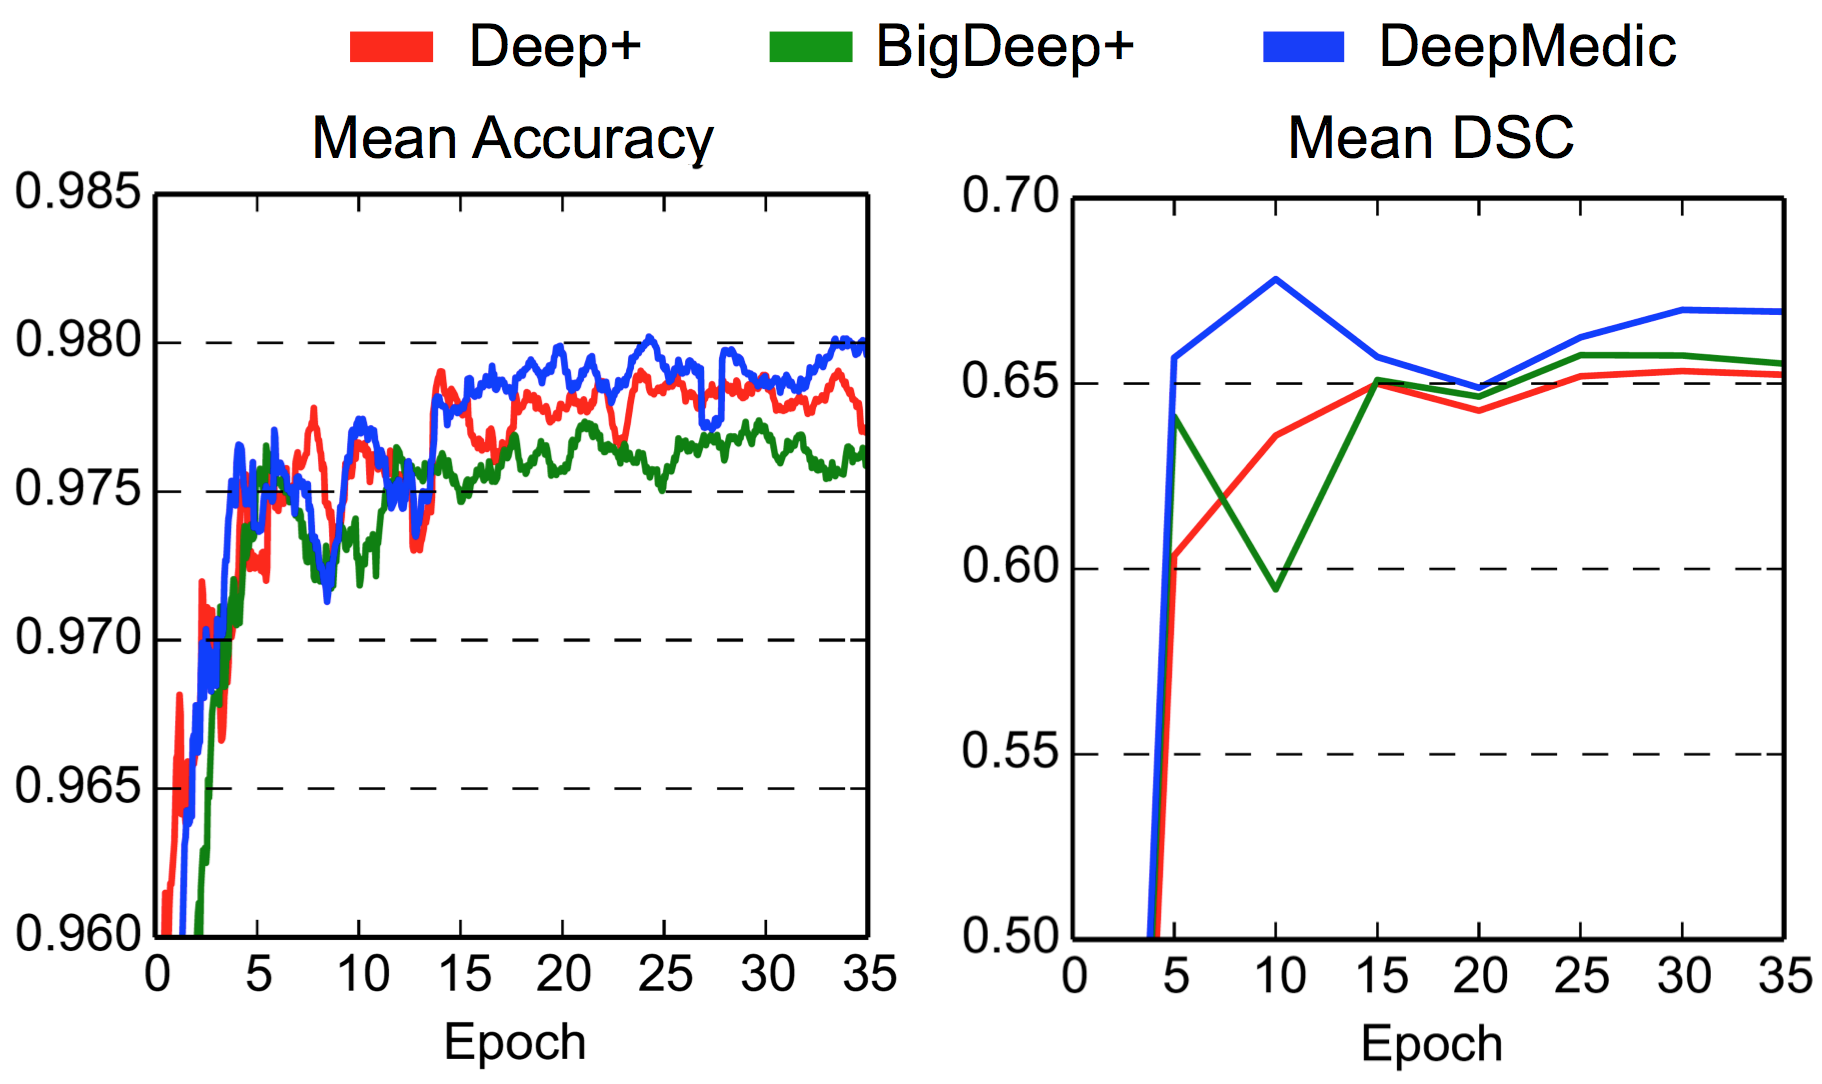
\includegraphics[clip=true, trim=0pt 0pt 0pt 0pt, width=1.0\textwidth]{figures/validationOfArchitecture/multiscale/figureToPut.png}
\end{subfigure}
\caption{Mean accuracy over validation samples and DSC for the segmentation of the validation images, as obtained by a single-scale model (Deep\texttt{+}) and our dual pathway architecture (DeepMedic). We also trained a single-scale model with larger capacity (BigDeep\texttt{+}), similar to the capacity of DeepMedic. DeepMedic yields best performance by capturing greater context, while BigDeep\texttt{+} seems to suffer from over-fitting.
}
\label{fig:multiscaleExperiment}
\end{figure}
%\vspace{-1pt} %takes away some white space before figure

The final version of the proposed network architecture, referred to as \quot{DeepMedic}, is built by extending the Deep\texttt{+} model with a second convolutional pathway that is identical to the first one. Two hidden layers are added for combining the multi-scale features before the classification layer, resulting in a deep network of 11-layers (cf. Fig.~\ref{fig:cnnMultiscale}). The input segments to the second pathway are extracted from the images down-sampled by a factor of three. Thus, the network is capable of capturing context in a $51^3$ area of the original image through the $17^3$ receptive field of the lower-resolution pathway, while only doubling the computational and memory requirements over the single pathway CNN. In comparison, the most recent 2D CNN systems proposed for lesion segmentation (\cite{Havei2015Journal, pereira2015Brats}) have a receptive field limited to $33^2$ voxels.

%+210 to left and -210 to right if I want to move one subfigure.
\begin{figure}[!h]
%\vspace{-1pt} %takes away some white space before figure
\centering
\begin{subfigure}[b]{0.85\textwidth}
\centering
	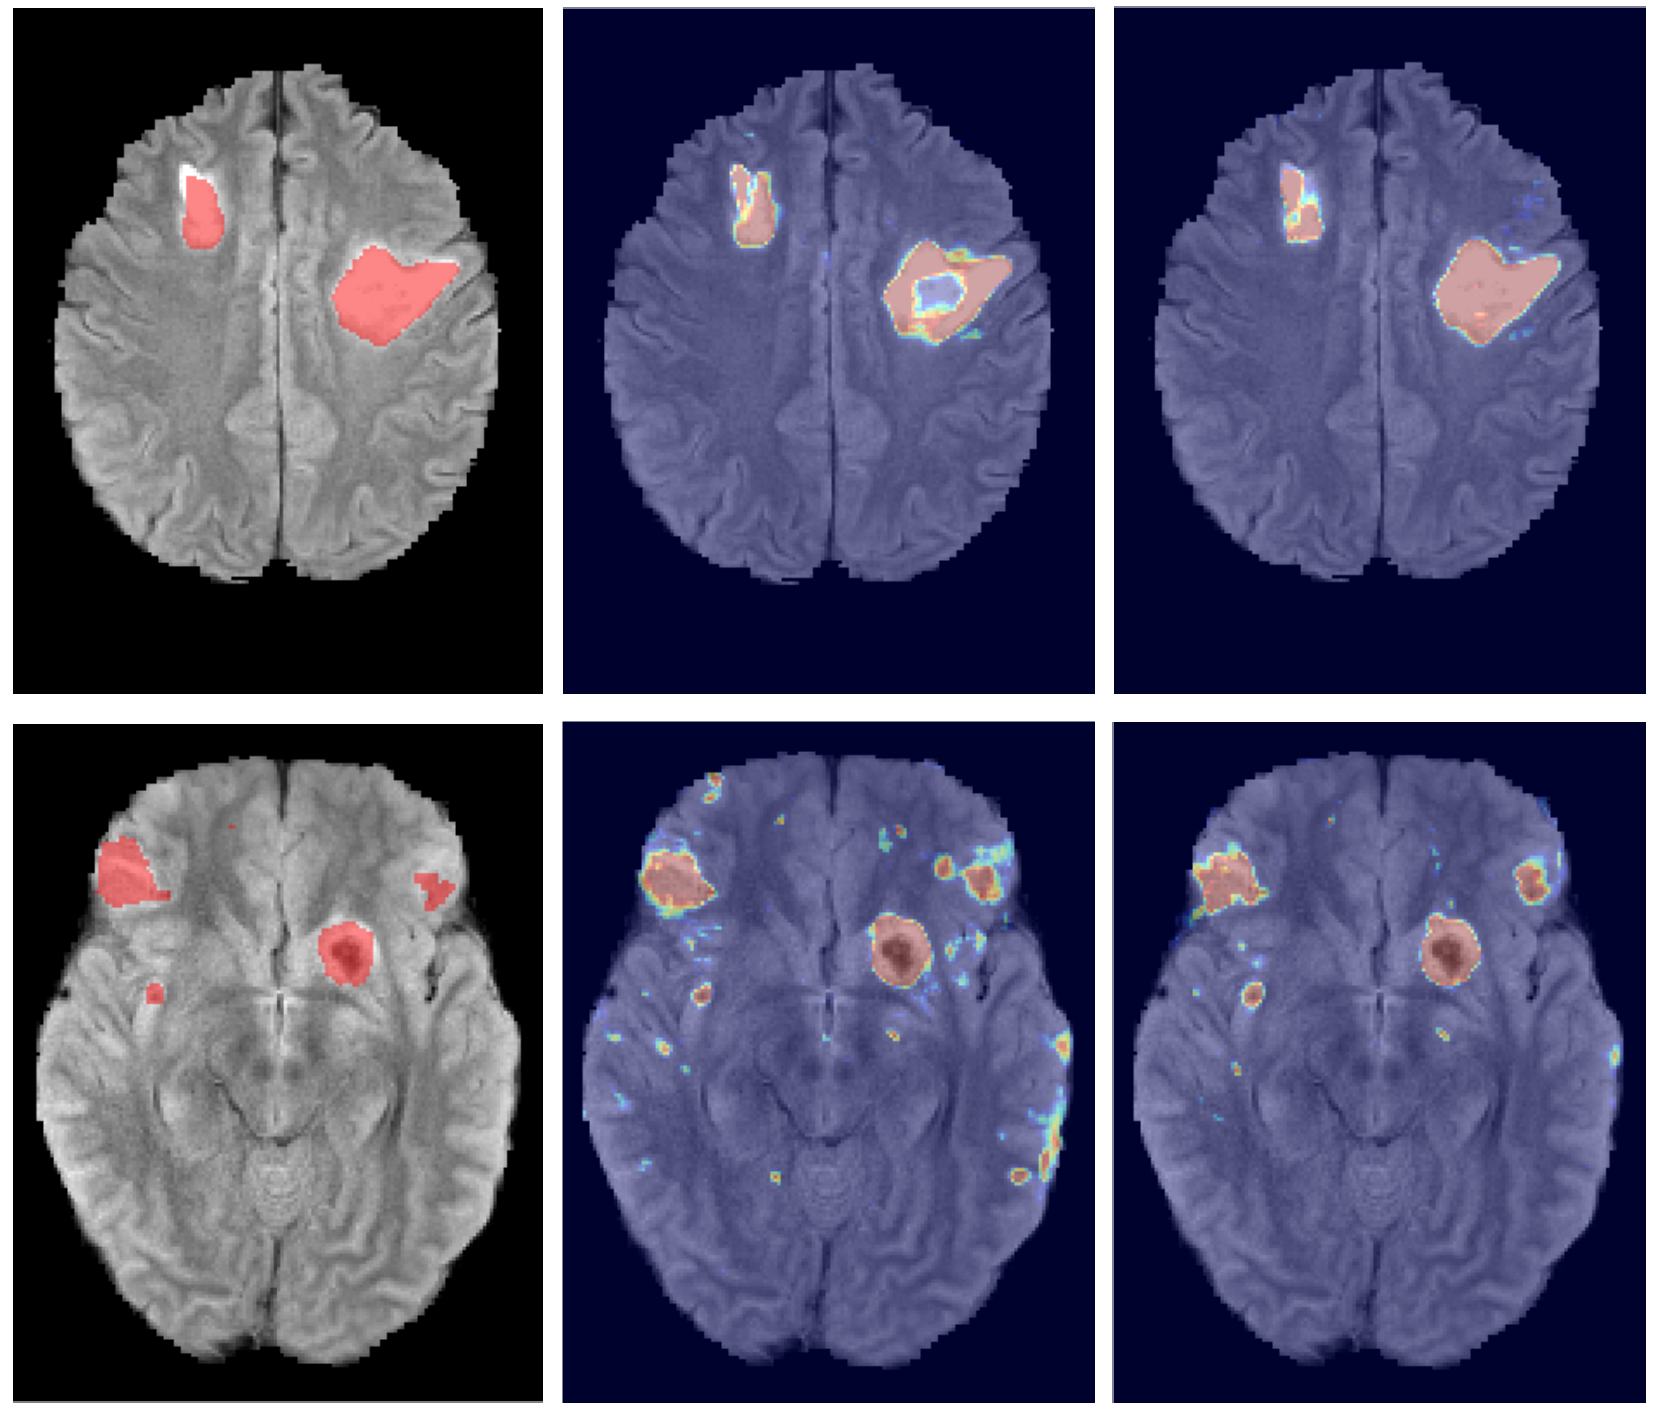
\includegraphics[clip=true, trim=0pt 0pt 0pt 0pt, width=1.0\textwidth]{figures/validationOfArchitecture/multiscale/qualitativeComparisonMultiscale/figureNew/multiscaleQual.png}
\end{subfigure}

\caption{(Rows) Two cases from the severe TBI dataset, showing representative improvements when using the multi-scale CNN approach. (Columns) From left to right: the MRI FLAIR sequence with the manually labeled lesions, predicted soft segmentation map obtained from a single-scale model (Deep\texttt{+}) and the prediction of the multi-scale DeepMedic model. The incorporation of greater context enables DeepMedic to identify when it processes an area within larger lesions (top). Spurious false positives are significantly reduced across the image on the bottom.}
\label{fig:qualitativeMultiscaleVal}
\end{figure}
%\vspace{-1pt} %takes away some white space before figure

Figure~\ref{fig:multiscaleExperiment} shows the improvement DeepMedic achieves over the single pathway model Deep\texttt{+}. In Fig.~\ref{fig:qualitativeMultiscaleVal} we show two representative visual examples of this improvement when using the multi-scale CNN. Finally, we confirm that the performance increase can be accounted to the additional context and not the additional capacity of DeepMedic. To this end, we build a big single-scale model by doubling the FMs at each of the 9-layers of Deep\texttt{+} and adding two hidden layers. This 11-layers deep and wide model, referred to as \quot{BigDeep\texttt{+}}, has the same number of parameters as DeepMedic. The performance of the model is not improved, while showing signs of over-fitting.

\subsection{Processing 3D in comparison to 2D Context}
\label{subsec:val3dContext}

Acquired brain MRI scans are often anisotropic. Such is the case for most sequences in our TBI dataset, which have been acquired with lower axial resolution, except for the isotropic MPRAGE. We perform a series of experiments to investigate the behaviour of 2D networks and assess the benefit of processing 3D context in this setting.

DeepMedic can be converted to 2D by setting the third dimension of each kernel to one. This way only information from the surrounding context on the axial plane influences the classification of each voxel. If 2D segments are given as input, the dimensionality of the feature maps decreases and so does the memory required. This allows developing 2D variants with increased width, depth and size of training batch with similar requirements as the 3D version, which are valid candidates for model selection in practical scenarios. We assess various configurations and present some representatives in Table \ref{subtab:netsConfig2d} along with their performance. Best segmentation among investigated 2D variants is achieved by a 19-layers, multi-scale network, reaching 61.5\% average DSC on the validation fold. The decline from the 66.6\% DSC achieved by the 3D version of DeepMedic indicates the importance of processing 3D context even in settings where most acquired sequences have low resolution along a certain axis.


% !TeX root=../journalDeepMedic.tex


%%%%%%%%%%%%%%%%%%%%%%%%%%%%%%%%%%%%%%%%%%%%%%%%%%%%%%%%%%%%%%
%%%%%%%%%%%%%%%%%%%% EVALUATION %%%%%%%%%%%%%%%%%%%%%%%%%%%%%%
%%%%%%%%%%%%%%%%%%%%%%%%%%%%%%%%%%%%%%%%%%%%%%%%%%%%%%%%%%%%%%

\section{Evaluation on Clinical Data}
\label{sec:evaluation}

The proposed system consisting of the DeepMedic CNN architecture, optionally coupled with a fully connected CRF, is evaluated on three lesion segmentation tasks including challenging clinical data from patients with traumatic brain injuries, brain tumors, and ischemic stroke. Quantitative evaluation and comparisons with state-of-the-art are reported for each of the tasks.

\subsection{Traumatic Brain Injuries}
\label{subsec:evalTbi}

\subsubsection{Material and Pre-Processing}
\label{subsubsec:materialTbi}

Sixty-six patients  with moderate-to-severe TBI who required admission to the Neurosciences Critical Care Unit at Addenbrooke's Hospital, Cambridge, UK, underwent imaging using a 3-Tesla Siemens Magnetom TIM Trio within the first week of injury. Ethical approval was obtained from the Local Research Ethics Committee (LREC 97/290) and written assent via consultee agreement was obtained for all patients. The structural MRI sequences that are used in this work are isotropic MPRAGE (1$mm\times$1$mm\times$1$mm$), axial FLAIR, T2 and Proton Density (PD) (0.7$mm\times$0.7$mm\times$5$mm$), and Gradient-Echo (GE) (0.86$mm\times$0.86$mm\times$5$mm$). All visible lesions were manually annotated on the FLAIR and GE sequences with separate labeling for each lesion type. In nine patients the presence of hyperintense white matter lesions that were felt to be chronic in nature were also annotated. Artifacts, for example, signal loss secondary to intraparenchymal pressure probes, were also noted. For the purpose of this study we focus on binary segmentation of all abnormalities within the brain tissue. Thus, we merged all classes that correspond to intra-cerebral abnormalities into a single \quot{lesion} label. Extra-cerebral pathologies such as epidural and subdural hematoma were treated as background. We excluded two datasets because of corrupted FLAIR images\ignore{13296, 17792}, two cases because no lesions were found\ignore{13776, 15883} and one case \ignore{11976} because of a major scanning artifact corrupting the images. This results in a total of 61 cases used for quantitative evaluation. Brain masks were obtained using the ROBEX tool (\cite{Iglesias2011}). All images were resampled to an isotropic $1mm^3$ resolution, with dimensions 193$\times$229$\times$193 and affinely registered (\cite{Studholme1999}) to MNI space using the atlas by \cite{Grabner2006}. No bias field correction was used as preliminary results showed that this can negatively affect lesion appearance. Image intensities were normalized to have zero-mean and unit variance, as it has been reported that this improves CNN results (\cite{Jarrett2009}).

\subsubsection{Experimental Setting}
\label{subsubsec:tbiExperimentalSetting}

\textbf{Network configuration and training:} The network architecture corresponds to the one described in Sec.~\ref{subsec:valMultiscale}, i.e. a dual-pathway, 11-layers deep CNN. The training data is augmented by adding images reflected along the sagittal axis. To make the network invariant to absolute intensities we also shift the intensities of each MR channel $c$ of every training segment by $i_c = r_c \sigma_c$. $r_c$ is sampled for every segment from $\mathcal{N}(0,0.1)$ and $\sigma_c$ is the standard deviation of intensities under the brain mask in the corresponding image. The network is regularized using dropout (\cite{hinton2012dropout}) with a rate of 2\% on all convolutional layers, which is in addition to a 50\% rate used on the last two layers. The network is evaluated with 5-fold cross-validation on the 61 subjects.

\textbf{CRF configuration:} The parameters of the fully connected CRF are determined in a configuration experiment using random-search and 15 randomly selected subjects from the TBI database with predictions from a preliminary version of the corresponding model. The 15 subjects are reshuffled into the 5-folds used for subsequent evaluation.

\textbf{Random Forest baseline:} We have done our best to set up a competitive baseline for comparison. We employ a context-sensitive Random Forest, similar to the model presented by \cite{Zikic2012} for brain tumors except that we apply the forest to the MR images without additional tissue specific priors. We train a forest with 50 trees and maximum depth of 30. Larger size did not improve results. Training data points are approximately equally sampled from lesion and background classes, with the optimal balance empirically chosen. Two hundred randomized cross-channel box features are evaluated at each split node with maximum offsets and box sizes of 20mm. The same folds of training and test sets are used as for our CNN approach.

\subsubsection{Results}
\label{subsec:resTbi}


\begin{table}[!h]
\centering
\scriptsize
\caption{Performance of \textit{DeepMedic} and an \textit{ensemble} of three networks on the TBI database. For comparison, we provide results for a Random Forest baseline. Values correspond to the mean (and standard deviation). Numbers in bold indicate significant improvement by the CRF post-processing, according to a two-sided, paired t-test on the DSC metric (*$p<5 \cdot 10^{-2}$, **$p<10^{-4}$).}
\label{table:accuracyTbiTrio}
\begin{tabular}{@{}llllll@{}}
\toprule
\multicolumn{1}{c}{}	& DSC			& Precision		& Sensitivity		& ASSD					& Haussdorf 	\\ \midrule
R. Forest			& 51.1(20.0)		& 50.1(24.4) 	& 60.1(15.8)			& 8.29(6.76)				& 64.17(15.98)	\\
R. Forest+CRF		& \textbf{54.8(18.5)**}	& 58.6(23.1)	& 56.9(17.4)		& 6.71(5.01)				& 59.45(15.52)	\\
DeepMedic			& 62.3(16.4)		& 65.3(18.8)		& 64.4(16.3)			& 4.24(2.64)				& 56.50(15.88)	\\
DeepMedic+CRF		& \textbf{63.0(16.3)**} & 67.7(18.2)	& 63.2(16.7)		& 4.02(2.54)				& 55.68(15.93)	\\
Ensemble				& 64.2(16.2)		& 67.7(18.3)		& 65.3(16.3)			& 3.88(2.33)				& 54.38(15.45)	\\
Ensemble+CRF			& \textbf{64.5(16.3)*} 	& 69.8(17.8)		& 63.9(16.7)		& 3.72(2.29)				&52.38(16.03)	\\
\bottomrule
\end{tabular}
\end{table}


Table \ref{table:accuracyTbiTrio} summarizes the results on TBI. Our CNN significantly outperforms the Random Forest baseline, while the relatively overall low DSC values indicate the difficulty of the task.  Due to randomness during training the local minima where a network converges are different between training sessions and some errors they produce differ (\cite{Choromanska2015}). To clear the unbiased errors of the network we form an \textit{ensemble} of three similar networks, aggregating their output by averaging. This ensemble yields better performance in all metrics but also allows us to investigate the behaviour of our network focusing only on the biased errors. Fig.~\ref{fig:evalTbiAccVsVol} shows the DSC obtained by the ensemble on each subject in relation to the manually segmented and predicted lesion volume. The network is capable of segmenting cases with very small lesions, although, performance is less robust in these cases as even small errors have large influence on the DSC metric. Investigation of the predicted lesion volume, which is an important biomarker for prognostication, shows that the network is neither biased towards the lesion nor background class, with promising results even on cases with very small lesions. Furthermore, we separately evaluate the influence of the post-processing with the fully connected CRF. As shown in Table \ref{table:accuracyTbiTrio}, the CRF yields improvements over all classifiers. Effects are more prominent when the performance of the primary segmenter degrades, which shows the robustness of this regulariser. Fig.~\ref{fig:evalTbiVisualQuality} shows three representative cases.

%+210 to left and -210 to right if I want to move one subfigure.

\begin{figure}[!ht]
%\vspace{-1pt} %takes away some white space before figure
\centering
\begin{subfigure}[b]{1.0\textwidth}
	\centering
	%\includegraphics[clip=true, trim=0pt 305pt 0pt 15pt, width=1.0\textwidth]{figures/evaluationSection/tbi/resultsVsLesionVolume/tbiAccuracyJournal.pdf}
	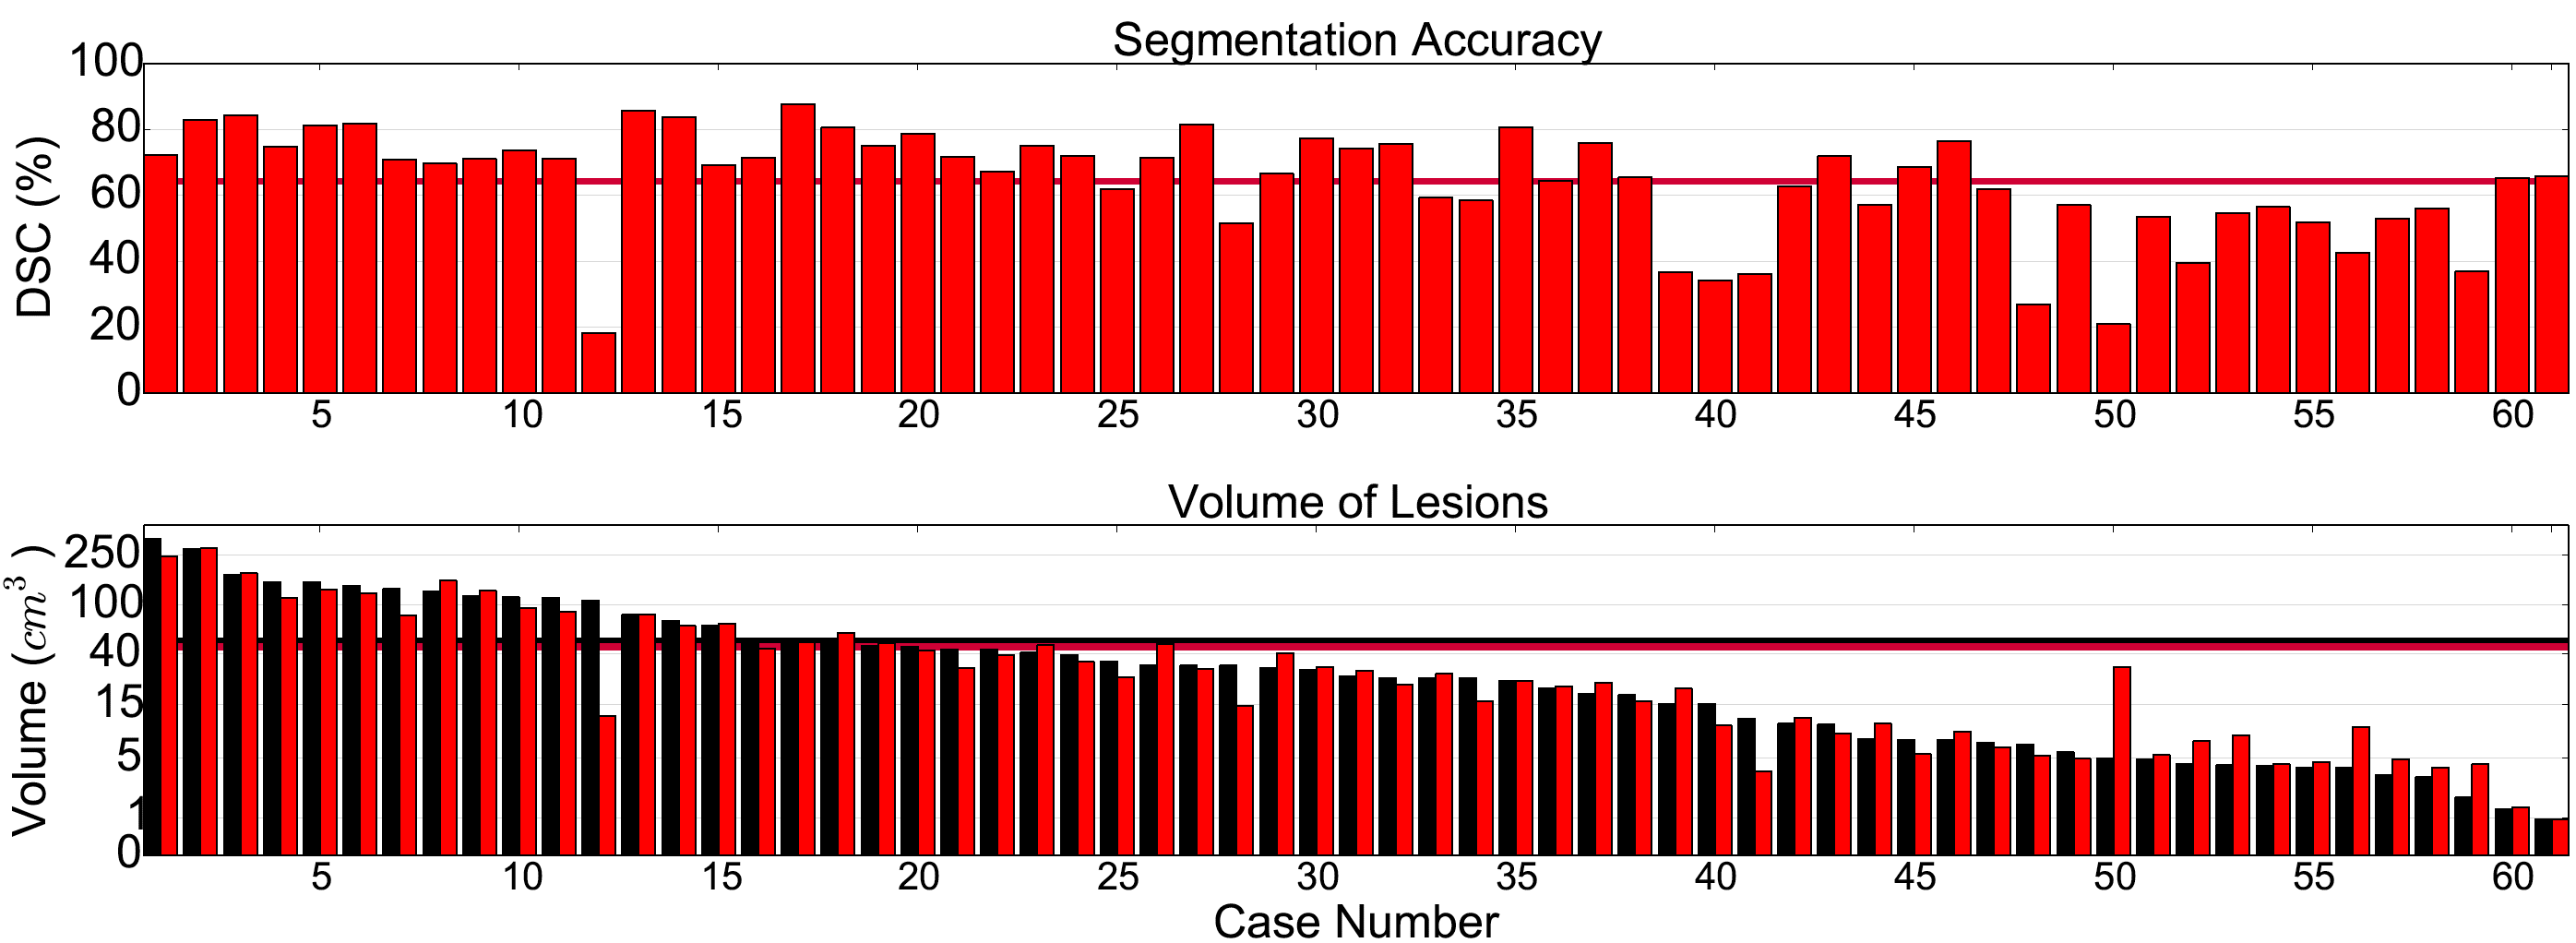
\includegraphics[clip=true, trim=0pt 0pt 0pt 0pt, width=1.0\textwidth]{figures/evaluationSection/tbi/resultsVsLesionVolume/tbiAccuracyJournal_nonReg.png}
\end{subfigure}
\vspace{-0pt} %takes away some white space before the caption
\caption{(Top) DSC achieved by our ensemble of three networks on each of the 61 TBI datasets. (Bottom) Manually segmented (black) and predicted lesion volumes (red). Note here the logarithmic scale. Continuous lines represent mean values. The outlying subject 12 presents small TBI lesions, which are successfully segmented, but also vascular ischemia. Because it is the only case in the database with the latter pathology, the networks fail to segment it as such lesion was not seen during training.}
\label{fig:evalTbiAccVsVol}
\vspace{-10pt}
\end{figure}
%\vspace{-1pt} %takes away some white space before figure

\begin{figure}[!ht]
%\vspace{-1pt} %takes away some white space before figure
\centering
\begin{subfigure}[b]{1.0\textwidth}
	\centering
	%\includegraphics[clip=true, trim=0pt 240pt 0pt 0pt, width=1.0\textwidth]{figures/evaluationSection/tbi/visualsQualitatively/visualsQualitatively3.png}
	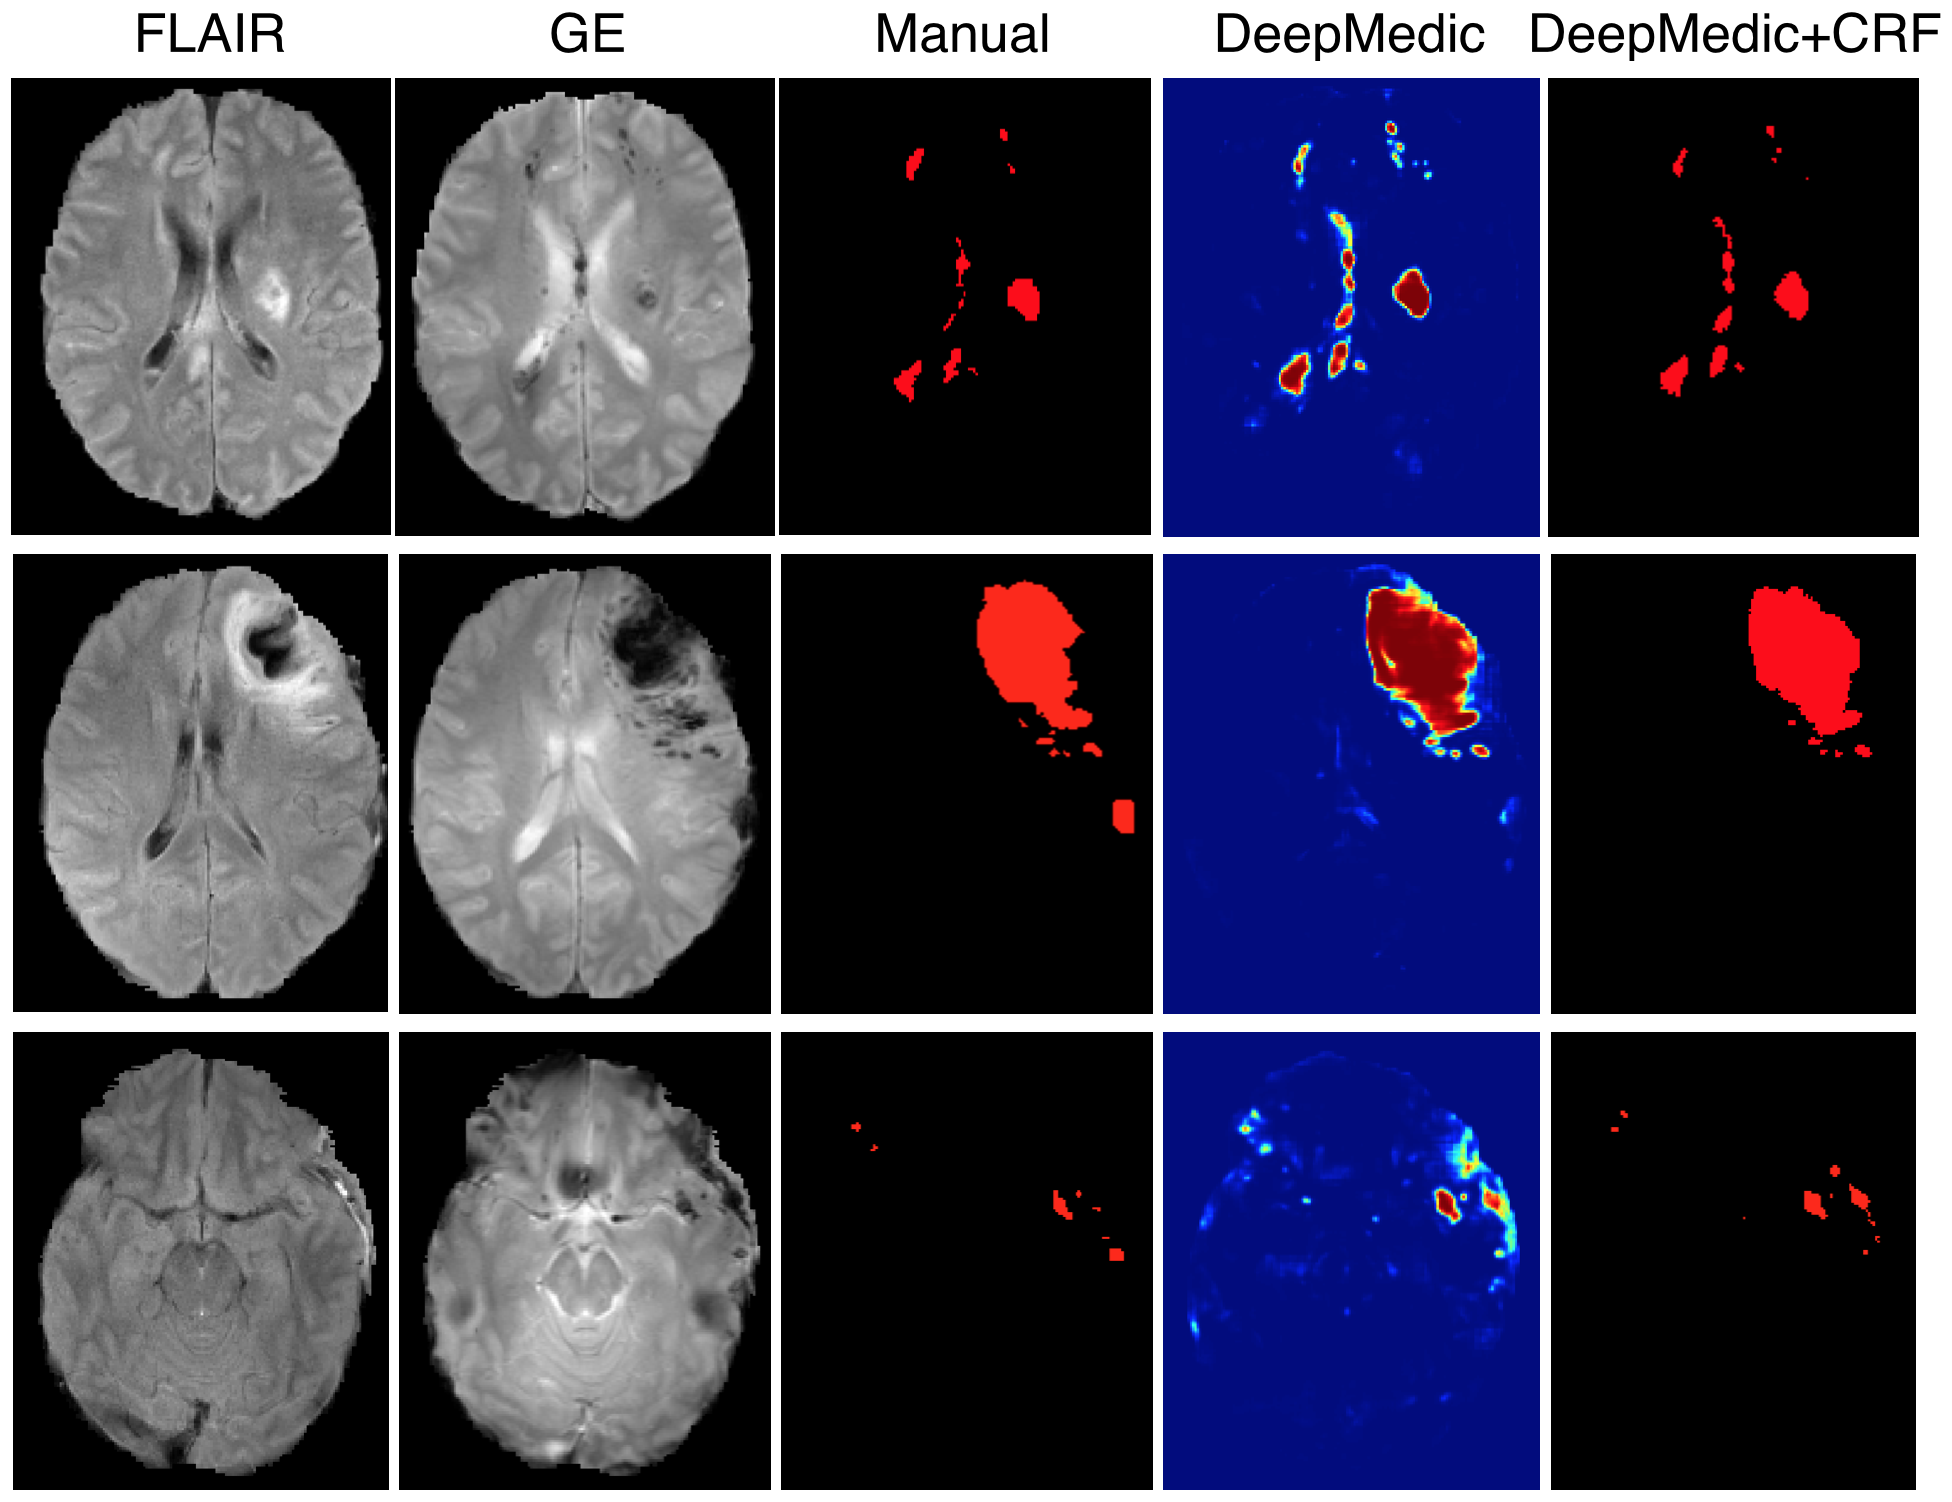
\includegraphics[clip=true, trim=0pt 0pt 0pt 0pt, width=1.0\textwidth]{figures/evaluationSection/tbi/visualsQualitatively/visualsQualitatively4.png}
\end{subfigure}
\vspace{-10pt} %takes away some white space before the caption
\caption{Three examples from the application of our system on the TBI database. It is capable of precise segmentation of both small and large lesions. Second row depicts one of the common mistakes observed. A contusion near the edge of the brain is under-segmented, possibly mistaken for background. Bottom row shows one of the worst cases, representative of the challenges in segmenting TBI. Post-surgical sub-dural debris is mistakenly captured by the brain mask. The network partly segments the abnormality, which is not a celebral lesion of interest.}
\label{fig:evalTbiVisualQuality}
\end{figure}
%\vspace{-1pt} %takes away some white space after figure


\subsection{Brain Tumor Segmentation}
\label{subsec:evalBrats}

\subsubsection{Material and Pre-Processing}

For brain tumors, we evaluate our system on the data from the 2015 Brain Tumor Segmentation Challenge (BRATS) (\cite{Menze2014}). The training set consists of 220 cases with high grade (HG) and 54 cases with low grade (LG) glioma for which corresponding reference segmentations are provided. The segmentations include the following tumor tissue classes: 1) necrotic core, 2) edema, 3) non-enhancing and 4) enhancing core. The test set consists of 110 cases of both HG and LG but the grade is not revealed. Reference segmentations for the test set are hidden and evaluation is carried out via an online system. For evaluation, the four predicted labels are merged into different sets of whole tumor (all four classes), the core (classes 1,3,4), and the enhancing tumor (class 4)\footnote{For interpretation of the results note that, to the best of our knowledge, cases where the \quot{enhancing tumor} class is not present in the manual segmentation are considered as zeros for the calculation of average performance by the evaluation platform, lowering the upper bound for this class.}. For each subject, four MRI sequences are available, FLAIR, T1, T1-contrast and T2. The datasets are pre-processed by the organizers and provided as skull-stripped, registered to a common space and resampled to isotropic $1mm^3$ resolution. Dimensions of each volume are 240$\times$240$\times$155. We add minimal pre-processing of normalizing the brain-tissue intensities of each sequence to have zero-mean and unit variance.


\subsubsection{Experimental Setting}

\textbf{Network configuration and training:} We modify the DeepMedic architecture to handle multi-class problems by extending the classification layer to five feature maps (four tumor classes plus background). The rest of the configuration remains unchanged. We enrich the dataset with sagittal reflections. Opposite to the experiments on TBI, we do not employ the intensity perturbation and dropout on convolutional layers, because the network should not require as much regularisation with this large database. The network is trained on image segments extracted with equal probability centred on the whole tumor and healthy tissue. The distribution of the classes captured by our training scheme is provided in \ref{app:distrTumorClassesTrain}.

To examine our network's behaviour, we first evaluate it on the training data of the challenge. For this, we run a 5-fold cross validation where each fold contains both HG and LG images. We then retrain the network using all training images, before applying it on the test data.

\textbf{CRF configuration:} For the multi-class problem it is challenging to find a global set of parameters for the CRF which can consistently improve the segmentation of all classes. So instead we merge the four predicted probability maps into a single \quot{whole tumor} map for CRF post-processing. The CRF then only refines the boundaries between tumor and background and additionally removes isolated false positives. Similarly to the experiments on TBI, the CRF is configured on a random subset of 44 HG and 18 LG training images, which are then reshuffled into the subsequent 5-fold cross validation. 

\subsubsection{Results}
\label{subsubsec:resBrats2015}



\begin{table}[!h]
\centering
\scriptsize
\caption{Average performance of our system on the training data of BRATS 2015 as computed on the online evaluation platform and comparison to other submissions visible at the time of manuscript submission. Presenting only teams that submitted more than half of the 274 cases. Numbers in bold indicate significant improvement by the CRF, according to a two-sided, paired t-test on the DSC metric (*$p<5\cdot 10^{-2}$, **$p<10^{-3}$). }
\label{table:onlineEvalBrats2015Training}
\begin{tabular}{@{}lllllllllll@{}}
\toprule
              & \multicolumn{3}{c}{DSC}  & \multicolumn{3}{c}{Precision} & \multicolumn{3}{c}{Sensitivity} &       \\ \cmidrule(lr){2-10}
              	& Whole & Core 	& Enh. 		& Whole   & Core  	& Enh.  & Whole & Core & Enh.   	& Cases \\ \midrule
              
Ensemble+CRF		& \textbf{90.1}*	&75.4	& \textbf{72.8}*	& 91.9	& 85.7	& 75.5	& 89.1	& 71.7	& 74.4	&274 \\
Ensemble			& 90.0			&75.5	& 72.8			& 90.3	& 85.5	& 75.4	& 90.4	& 71.9	& 74.3	&274 \\
DeepMedic+CRF	& \textbf{89.8}**&75.0	& \textbf{72.1}*	& 91.5	& 84.4	& 75.9	& 89.1	& 72.1	& 72	.5	&274 \\
DeepMedic		& 89.7			& 75.0	& 72.0			& 89.7	& 84.2	& 75.6	& 90.5	& 72.3	& 72.5	&274 \\

bakas1		 	& 88				& 77		& 68				& 90		& 84		& 68		& 89		& 76		& 75		&186\\
peres1		 	& 87				& 73		& 68				& 89		& 74		& 72		& 86		& 77		& 70		&274\\
anon1		 	& 84				& 67		& 55				& 90		& 76		& 59		& 82		& 68		& 61		&274\\
thirs1		 	& 80				& 66		& 58				& 84		& 71		& 53 	& 79		& 66		& 74		&267\\
peyrj			& 80				& 60		& 57				& 87		& 79		& 59		& 77		& 53		& 60		&274\\
\bottomrule
\end{tabular}
\end{table}

Quantitative results from the application of the DeepMedic, the CRF and an ensemble of three similar networks on the training data are presented in Table \ref{table:onlineEvalBrats2015Training}. The latter two offer an improvement, albeit fairly small since the performance of DeepMedic is already rather high in this task. Also shown are results from previous works, as reported on the online evaluation platform. Various settings may vary among submissions, such as the pre-processing pipeline or the number of folds used for cross-validation. Still it appears that our system performs favourably compared to previous state-of-the-art, including the semi-automatic system of \cite{bakas2015Brats} (bakas1) who won the latest challenge and the method of \cite{pereira2015Brats} (peres1), which is based on grade-specific 2D CNNs and requires visual inspection of the tumor and identification of the grade by the user prior to segmentation. Examples of segmentations obtained with our method are shown in Fig.~\ref{fig:evalBratsVisualQuality}. DeepMedic behaves very well in preserving the hierarchical structure of the tumor, which we account to the large context processed by our multi-scale network.



Table~\ref{table:onlineEvalBrats2015Testing} shows the results of our method on the BRATS test data. Results of other submissions are not accessible. The decrease in performance is possibly due to the the inclusion of test images that vary significantly from the training data, such as cases acquired in clinical centers that did not provide any of the training images, something that was confirmed by the organisers. Note that performance gains obtained with the CRF are larger in this case. This indicates not only that its configuration has not overfitted to the training database but also that the CRF is robust to factors of variation between acquisition sites, which complements nicely the more sensitive CNN.


\begin{table}[!h]
\centering
\scriptsize
\caption{Average performance of our system on the 110 test cases of BRATS 2015, as computed on the online evaluation platform. Numbers in bold indicate significant improvement by the CRF, according to a two-sided, paired t-test on the DSC metric (*$p<5\cdot 10^{-2}$, **$p<10^{-3}$). The decrease of the mean DSC by the CRF and the ensemble for the \quot{Core} class was not found significant.}
\label{table:onlineEvalBrats2015Testing}
\begin{tabular}{@{}llllllllll@{}}
\toprule
              & \multicolumn{3}{c}{DSC}  & \multicolumn{3}{c}{Precision} & \multicolumn{3}{c}{Sensitivity} \\ \cmidrule(l){2-10} 
              & Whole 			& Core & Enh. 			& Whole   & Core   & Enh.	& Whole    & Core   & Enh.   \\ \midrule

DeepMedic     & 83.6  			& 67.4 & 62.9      		& 82.3    & 84.6   & 64.0    & 88.5     & 61.6   & 65.6      \\
DeepMedic+CRF & \textbf{84.7}** 	& 67.0 & 62.9      		& 85.0    & 84.8   & 63.4    & 87.6     & 60.7   & 66.2      \\
Ensemble      & 84.5  			& 66.7 & 63.3      		& 83.3    & 86.1   & 63.2    & 88.9     & 59.9   & 67.3      \\
Ensemble+CRF  & \textbf{84.9}** 	& 66.7 & \textbf{63.4}* 	& 85.3    & 86.1   & 63.4    & 87.7     & 60.0   & 67.4		\\
\bottomrule
\end{tabular}
\end{table}

\begin{figure}[!h]
%\vspace{-1pt} %takes away some white space before figure
\centering
\begin{subfigure}[b]{1.0\textwidth}
	\centering
	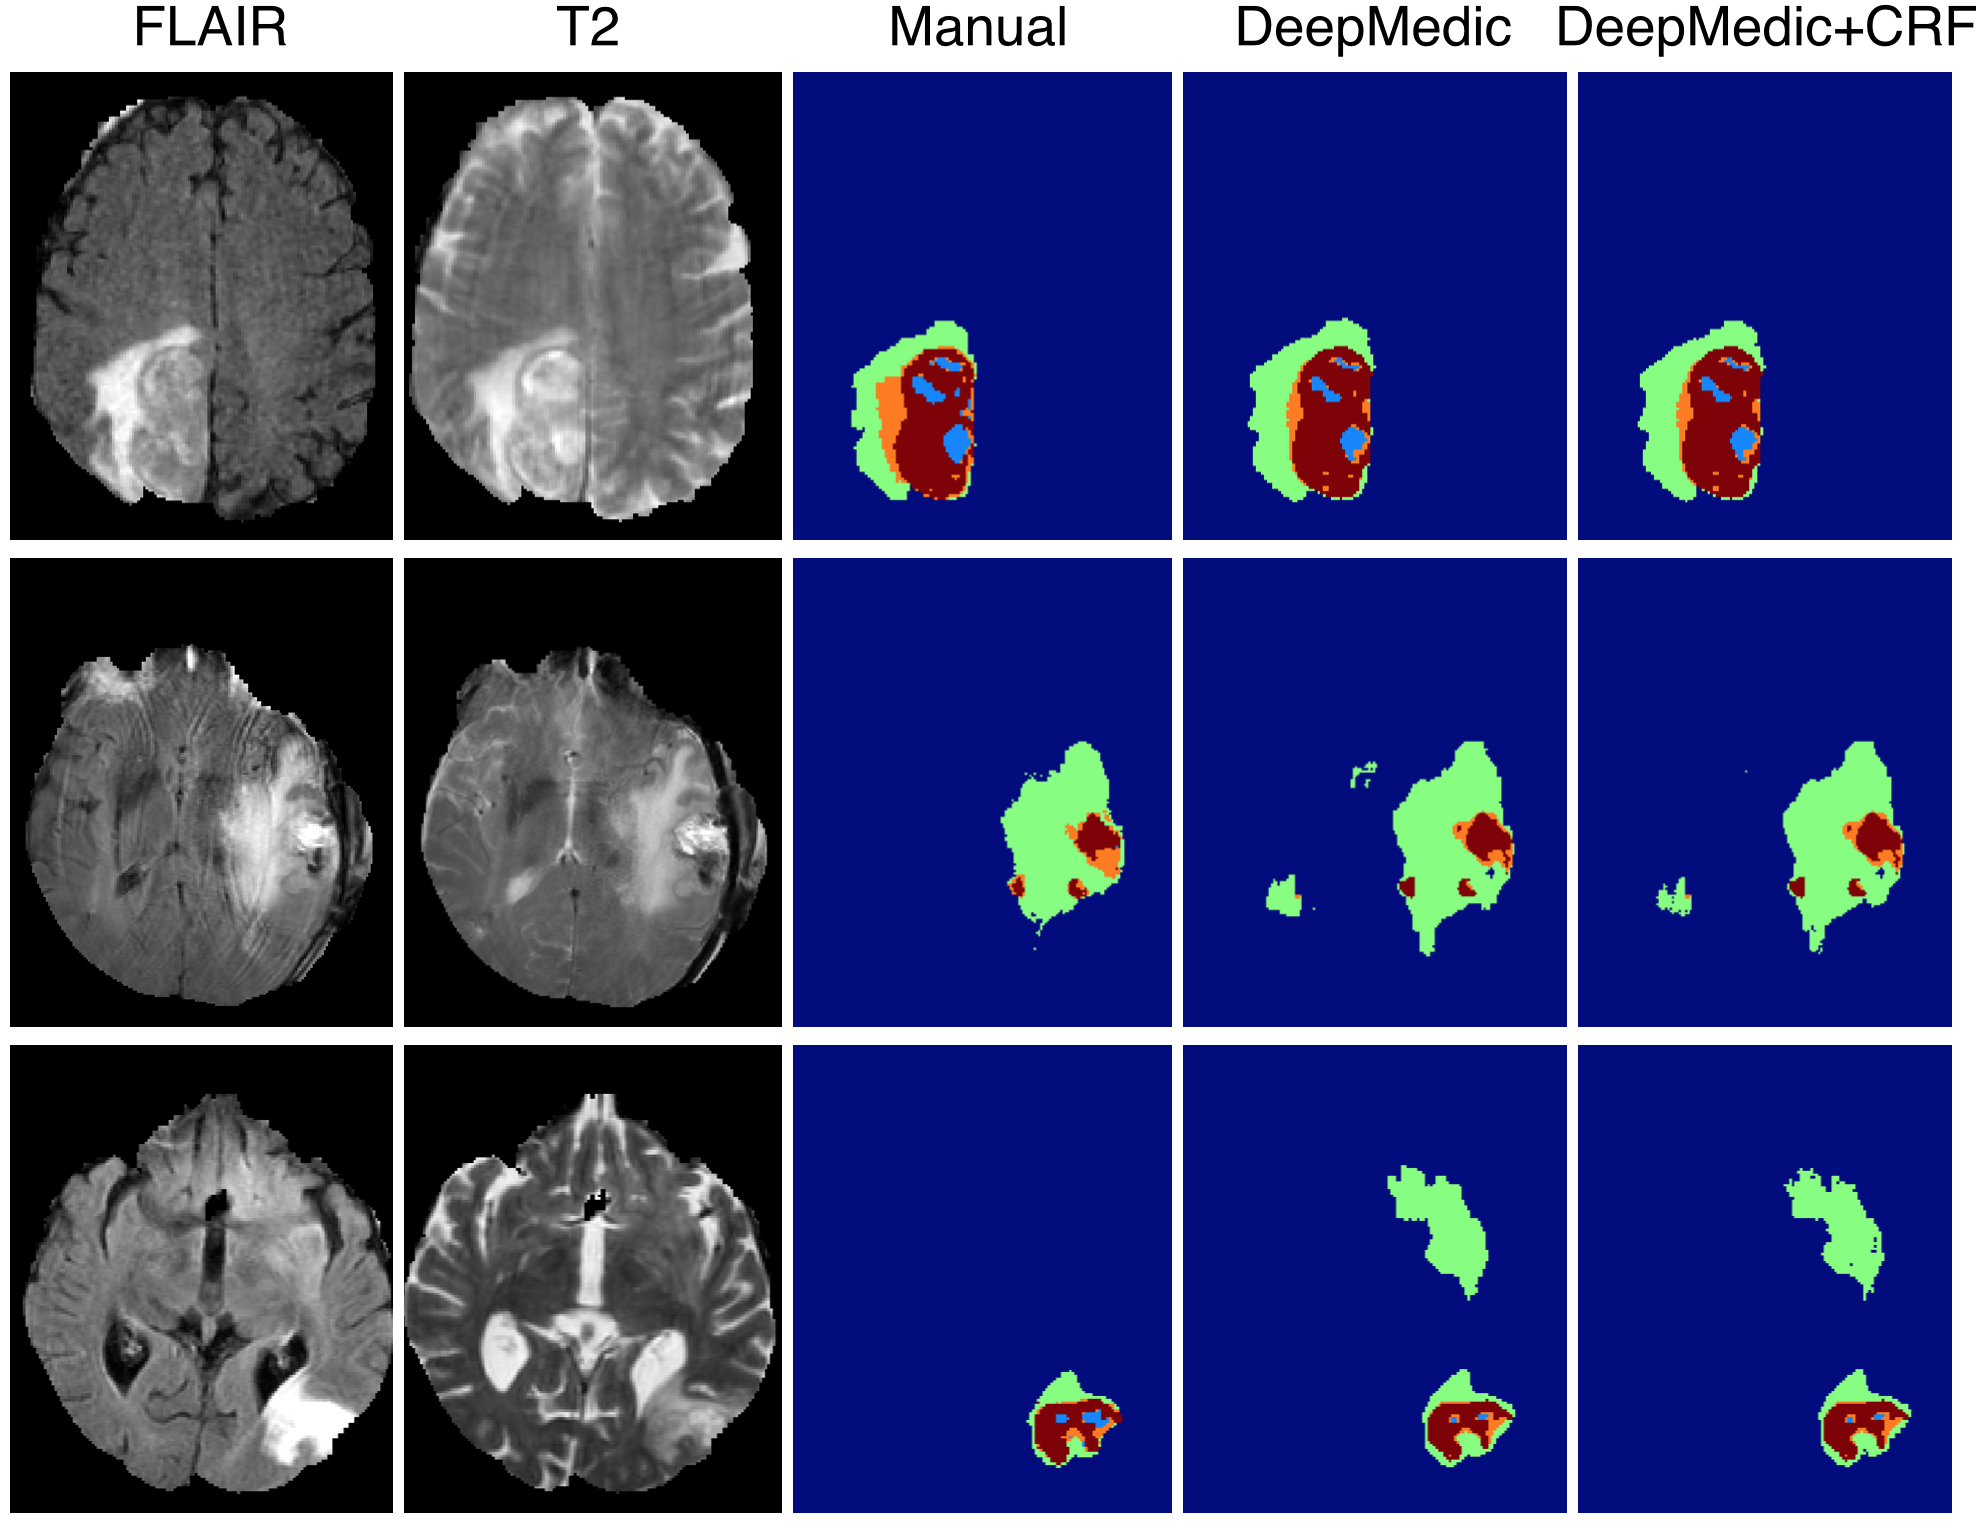
\includegraphics[clip=true, trim=0pt 0pt 0pt 0pt, width=1.0\textwidth]{figures/evaluationSection/brats/qualitative/bratsQualitatively.png}
\end{subfigure}
\vspace{-0pt} %takes away some white space before the caption
\caption{Examples of DeepMedic's segmentation from its evaluation on the training datasets of BRATS 2015. cyan: necrotic core, green: oedema, orange: non-enhancing core, red: enhancing core. (top and middle) Satisfying segmentation of the tumor, regardless motion artefacts in certain sequences. (bottom) One of the worst cases of over-segmentation observed. False segmentation of FLAIR hyper-intensities as oedema constitutes the most common error of DeepMedic.}
\label{fig:evalBratsVisualQuality}
\end{figure}
%\vspace{-1pt} %takes away some white space after figure



\subsection{Ischemic Stroke Lesion Segmentation}
\label{subsec:evalIsles}

\subsubsection{Material and Pre-Processing}

We participated in the 2015 Ischemic Stroke Lesion Segmentation (ISLES) challenge, where our system achieved the best results among all participants on sub-acute ischemic stroke lesions (\cite{maier2017isles}). In the training phase of the challenge, 28 datasets have been made available, along with manual segmentations. Each dataset included T1, T1-contrast, FLAIR and DWI sequences. All images were provided as skull-stripped and resampled to isotropic $1mm^3$ voxel resolution. Each volume is of size 230$\times$230$\times$154. In the testing stage, teams were provided with 36 datasets for evaluation. The test data were acquired in two clinical centers, with one of them being the same that provided all training images. Corresponding expert segmentations were hidden and results had to be submitted to an online evaluation platform. Similar to BRATS, the only pre-processing that we applied is the normalization of each image to the zero-mean and unit variance.

\subsubsection{Experimental Setting}

\textbf{Network Configuration and Training:} The configuration of the network employed is described in \cite{kamnitsas2015Isles}. The main difference with the configuration used for TBI and tumors as employed above is the relatively smaller number of FMs in the low-resolution pathway. This choice should not significantly influence accuracy on the generally small SISS lesions but it allowed us to lower the computational cost.

Similar to the other experiments, we evaluate our network with a 5-fold cross validation on the training datasets. We use data augmentation with sagittal reflections. For the testing phase of the challenge, we trained an ensemble of three networks on all training cases and aggregate their predictions by averaging.

\textbf{CRF configuration:} The parameters of the CRF were configured via a random search on the whole training dataset.

\subsubsection{Results}
\label{subsubsec:resIsles2015}

The performance of our system on the training data is shown in Table~\ref{table:accuracyIslesTraining}. Significant improvement is achieved by the structural regularisation offered by the CRF, although it could be partially accounted for by overfitting the training data during the CRF's configuration. Examples for visual inspection are shown in Fig.~\ref{fig:evalIslesVisualQuality}.

\begin{table}[!h]
\centering
\scriptsize
\caption{Performance of our system on the training data of the ISLES-SISS 2015 competition. Values correspond to the mean (and standard deviation). Numbers in bold indicate significant improvement by the CRF, according to a two-sided, paired t-test on the DSC metric ($p<10^{-2}$).}
\label{table:accuracyIslesTraining}
\begin{tabular}{@{}llllll@{}}
\toprule
\multicolumn{1}{c}{}		& DSC				& Precision		& Sensitivity	& ASSD			& Haussdorf 	\\ \midrule
DeepMedic				& 64(23)		 		& 68(24)			& 65(23)			& 6.99(9.91)		& 73.32(26.03)	\\
DeepMedic+CRF			& \textbf{66(24)}	& 77(24)			& 63(25)			& 5.00(10.33	)	& 55.93(28.55)	\\
\bottomrule
\end{tabular}
\end{table}


\begin{table}[!h]
\centering
\scriptsize
\caption{Our ensemble of three networks, coupled with the fully connected CRF obtained overall best performance among all participants in the testing stage of the ISLES-SISS 2015 challenge. Shown is the performance of our pipeline along with the second and third entries. Values correspond to the mean (and standard deviation).}
\label{table:accuracyIslesTesting}
\begin{tabular}{@{}llllll@{}}
\toprule
\multicolumn{1}{c}{}		& DSC		& Precision		& Sensitivity	& ASSD			& Haussdorf 	\\ \midrule
kamnk1(ours)				& 59(31)		& 68(33)			& 60(27) 		& 7.87(12.63)	& 39.61(30.68)	\\
fengc1					& 55(30)		& 64(31)			& 57(33)	 		& 8.13(15.15)	& 25.02(22.02)	\\
halmh1					& 47(32)		& 47(34)			& 56(33)	 		& 14.61(20.17)	& 46.26(34.81)	\\
\bottomrule
\end{tabular}
\end{table}

For the testing phase of the challenge we formed an ensemble of three networks, coupled with the fully connected CRF. Our submission ranked first, indicating superior performance on this challenging task among 14 submissions. Table~\ref{table:accuracyIslesTesting} shows our results, along with the other two top entries (\cite{feng2015Isles,halme2015Isles}). Among the other participating methods was the CNN of \cite{Havei2015Journal} with 3 layers of 2D convolutions. That method perfomed less well on this challenging task (\cite{maier2017isles}). This points out the advantage offered by 3D context, the large field of view of DeepMedic thanks to multi-scale processing and the representational power of deeper networks. It is important to note the decrease of performance in comparison to the training set. All methods performed worse on the data coming from the second clinical center, including the method of \cite{feng2015Isles} that is not machine-learning based. This highlights a general difficulty with current approaches when applied on multi-center data.

\begin{figure}[!h]
%\vspace{-1pt} %takes away some white space before figure
\centering
\begin{subfigure}[b]{1.0\textwidth}
	\centering
	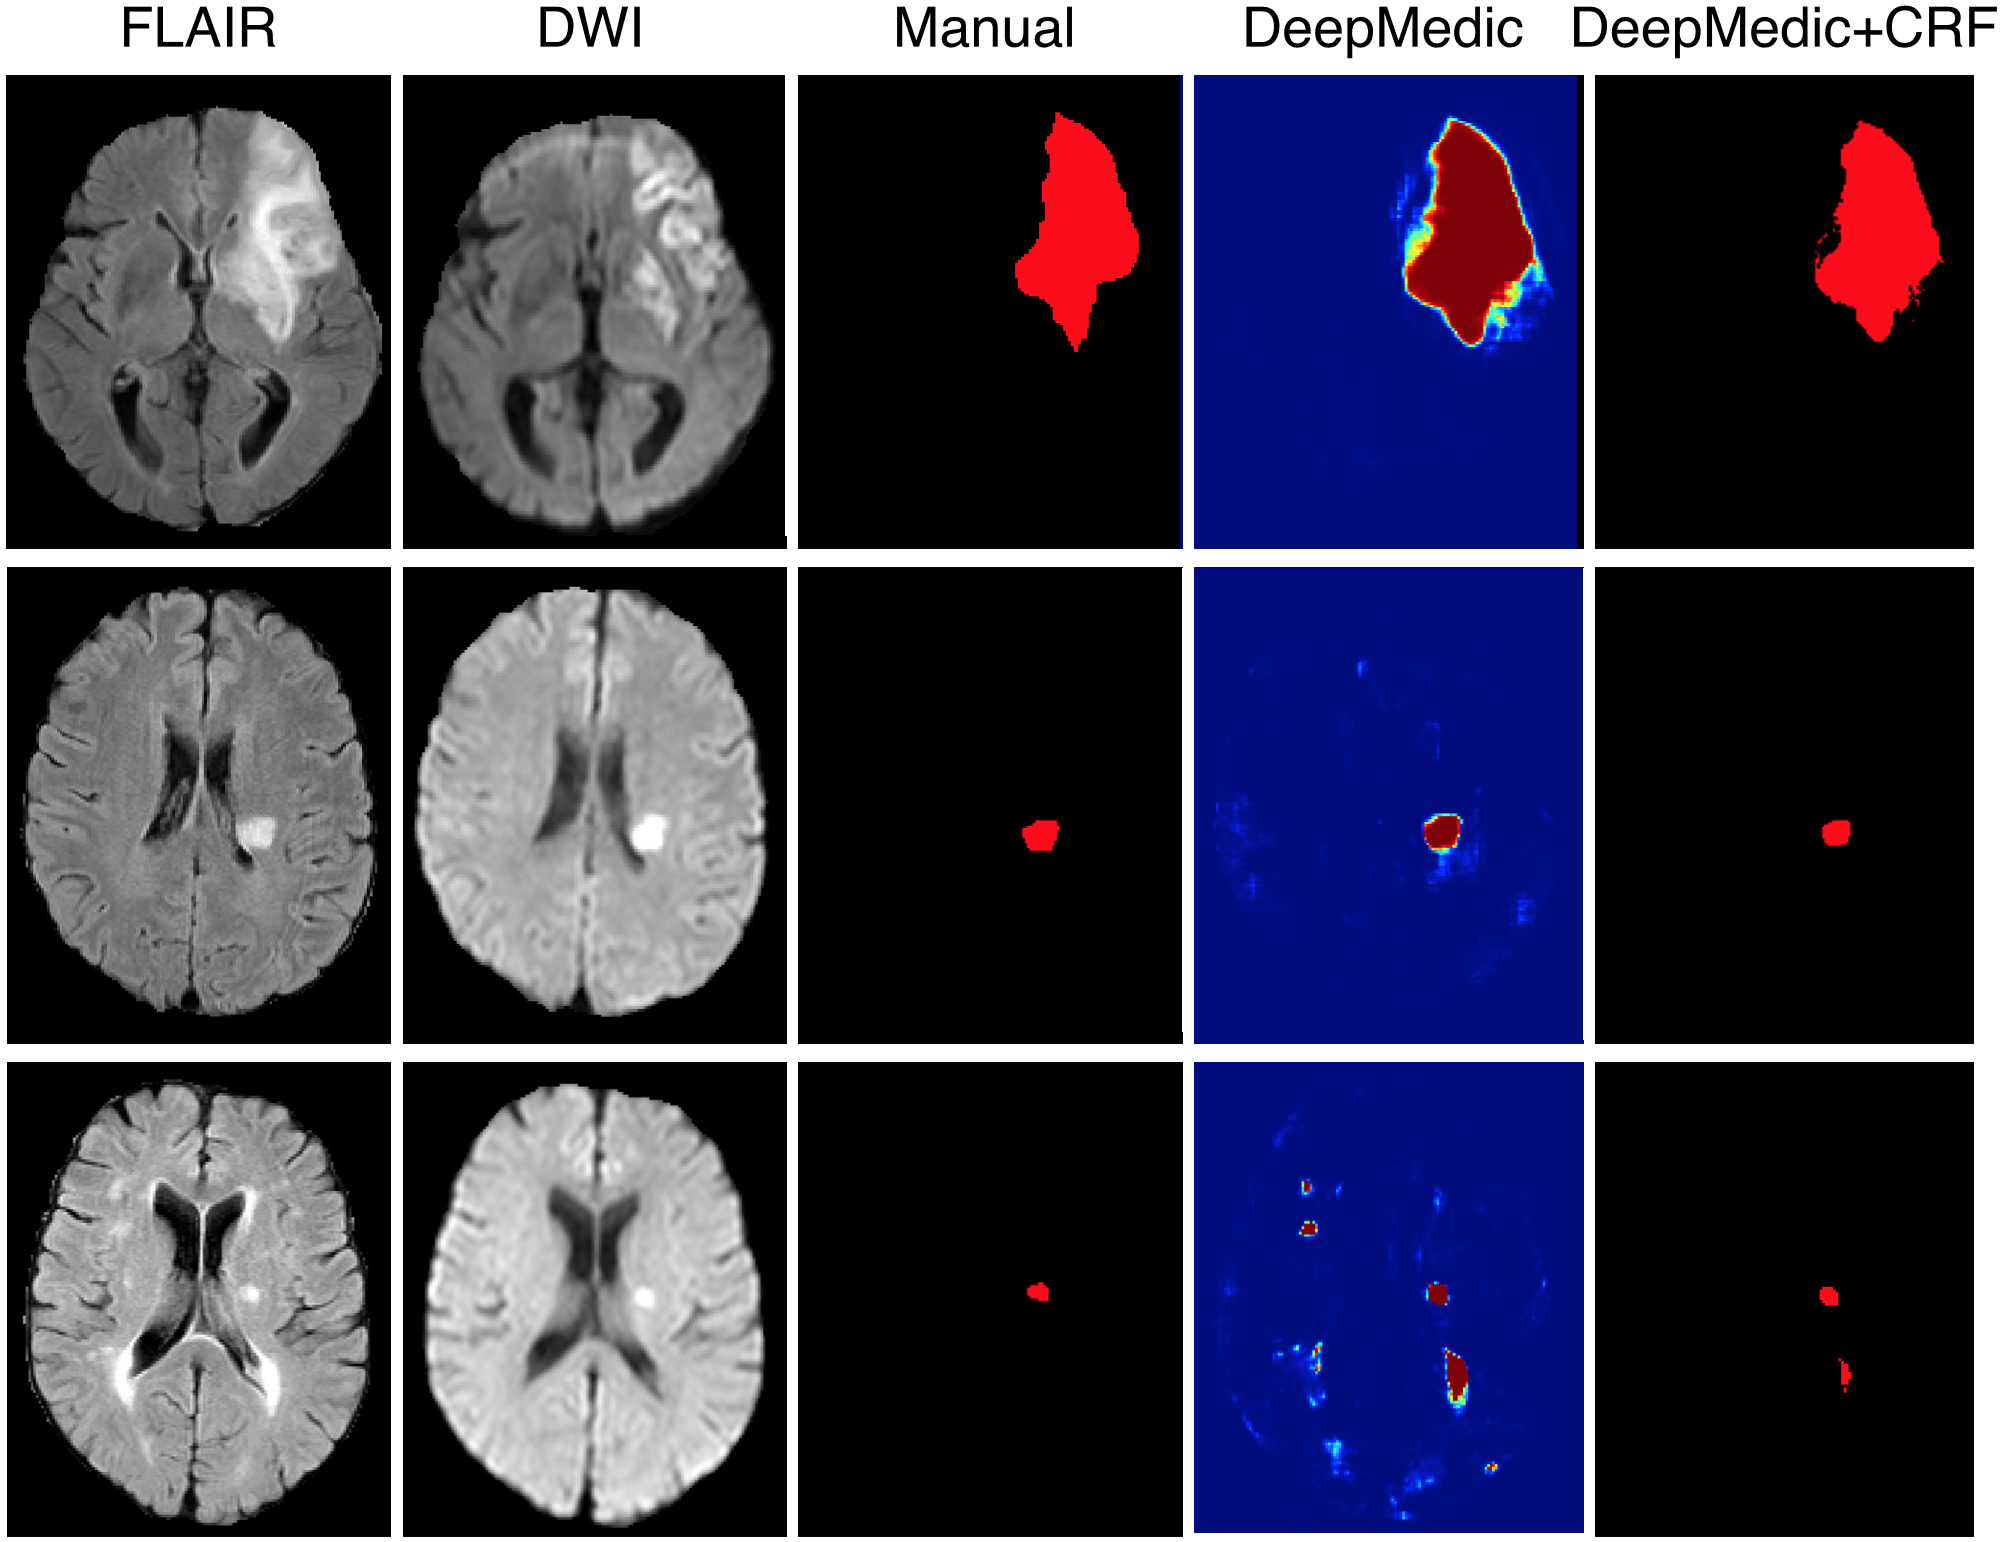
\includegraphics[clip=true, trim=0pt 0pt 0pt 0pt, width=1.0\textwidth]{figures/evaluationSection/isles/qualitative/isles15TrainingQualitatively.png}
\end{subfigure}
\vspace{-0pt} %takes away some white space before the caption
\caption{Examples of segmentations performed by our system on the training datasets of (SISS) ISLES 2015. (top and middle) The system is capable of satisfying segmentation of both large and smaller lesions. (bottom) Common mistakes are performed due to the challenge of differentiating stroke lesions from White Matter lesions. }
\label{fig:evalIslesVisualQuality}
\end{figure}
%\vspace{-1pt} %takes away some white space after figure

\subsection{Implementation Details}
 
Our CNN is implemented using the Theano library (\cite{Bastien-Theano-2012}). Each training session requires approximately one day on an NVIDIA GTX Titan X GPU using cuDNN v5.0. The efficient architecture of DeepMedic also allows models to be trained on GPUs with only 3GB of memory. Note that although dimensions of the volumes in the processed databases do not allow dense training on whole volumes for this size of network, dense inference on a whole volume is still possible, as it requires only a forward-pass and thus less memory. In this fashion segmentation of a volume takes less than 30 seconds but requires 12 GB of GPU memory. Tiling the volume into multiple segments of size $35^3$ allows inference on 3 GB GPUs in less than three minutes.

Our 3D fully connected CRF is implemented by extending the original source code by \cite{Krahenbuhl2013}. A CPU implementation is fast, capable of processing a five-channel brain scan in under three minutes. Further speed-up could be achieved with a GPU implementation, but was not found necessary in the scope of this work.


\section{Discussion}
\label{sec:discussion}

The accuracy on the CKP set shows that the chosen approach is robust, misclassification usually occurs on pictures which are the first few instances of an emotion sequence. Often a neutral facial expression is depicted in those frames. Thus those misclassifications are not necessarily an error in the approach, but in the data selection. Other than that no major problem could be detected. The emotion \textit{Surprise} is often confused with \textit{Disgust} with a rate of 0.045\% which is the highest. Of those images, where an emotion is present, only few are wrongly classified.\\ 


As there is no consent for the misclassified images, they cannot be depicted here. However some unique names are provided. \\
Image S119\_001\_00000010 is classified as \textit{Fear} while the annotated emotion corresponds to \textit{Surprise}. The image depicts a person with a wide open mouth and open eyes. Pictures representing \textit{Surprise} are often very similar, since the persons also have wide open mouths and eyes. In image S032\_004\_00000014 the targeted label \textit{Fear} is confused with \textit{Anger}. While the mouth region in pictures with \textit{Anger} differ, the eye regions are alike, since in both situations the eyes and eyebrows are contracted.\\
Similar effects are experienced when dealing with the MMI Dataset. Since the first two frames are discarded most pictures with neutral positions are excluded. In few images a neutral position can still be found which gives rise to errors. For the same reason as the CKP set images will not be displayed. Due to the approach to extract images of the videos, a unique identifier for the misclassified image cannot be provided.\\
The top confusions are observed for \textit{Fear} and \textit{Surprise} with a rate of 0.0159\% where \textit{Fear} is wrongly misclassified as \textit{Surprise}. Session 1937 shows a woman displaying \textit{Fear} but it is classified as \textit{Surprise}. Both share common features like similar eye and mouth movement. In both emotions, participants move the head slightly backwards. This can be identified by wrinkled skin. The second most confusion rate, \textit{Surprise} being mistaken as \textit{Sadness}, is mostly based on neutral position images. Although the first two images are not used, some selected frames still do not contain an emotion. In Session 1985 \textit{Surprise} is being mistaken as \textit{Sadness}. The image depicts a man with his mouth being slightly curved, making him look sad.\\

DeXpression extracts features and uses them to classify images, but in very few cases the emotions are confused. This happens, as discussed, usually in pictures depicting no emotion. DeXpression performs very well on both tested sets, if an emotion is present.



%!TEX root = pixelrnn.tex

\section*{Acknowledgements}

The authors would like to thank Shakir Mohamed and Guillaume Desjardins for helpful input on this paper and Lucas Theis, Alex Graves, Karen Simonyan, Lasse Espeholt, Danilo Rezende, Karol Gregor and Ivo Danihelka for insightful discussions.


%%%%%%%%%%%%%%%%%%%%%%%%%%%%%%%%%%%%%%%%%%%%%%%%%%%%%%%%%%%%%%
%%%%%%%%%%%%%%%%%%%% APPENDIX %%%%%%%%%%%%%%%%%%%%%%%%%%%%%%
%%%%%%%%%%%%%%%%%%%%%%%%%%%%%%%%%%%%%%%%%%%%%%%%%%%%%%%%%%%%%%

\appendix

%\section*{Appendix}

\section{Additional Details on Multi-Scale Processing}
\label{app:detailsMultiscale}

The integration of multi-scale parallel pathways in architectures that use solely unary kernel strides, such as the proposed, was described in Sec.~\ref{subsec:multiscaleCnn}. The required up-sampling of the low-resolution features was performed with simple repetition in our experiments. This was found sufficient, with the following hidden layers learning to combine the multi-scale features. In the case of architectures with strides greater than unary, the last convolutional layers of the two pathways, $L1$ and $L2$, have receptive fields $\boldsymbol{\varphi}_{L1}$ and $\boldsymbol{\varphi}_{L2}$ with strides $\boldsymbol{\tau}_{L1}$ and $\boldsymbol{\tau}_{L2}$ respectively. To preserve spatial correspondence of the multi-scale features and enable the network for dense inference, the dimensions of the input segments should be chosen such that the FMs in $L2$ can be brought to the dimensions of the FMs in $L1$ after sequential resampling by $\uparrow \boldsymbol{\tau}_{L2}$, $\uparrow F_D$, $\downarrow \boldsymbol{\tau}_{L1}$ or equivalent combinations. Here $\uparrow$ and $\downarrow$ represent up- and down-sampling by the given factor. Because they are more reliant on these operations, utilization of more elaborate, learnt upsampling schemes (\cite{Long2014, Ronneberger2015, Noh2015}) should be beneficial in such networks.


\section{Additional Details on Network Configurations}
\label{app:detailsConfig}

\textbf{3D Networks:} The main description of our system is presented in Sec.~\ref{sec:segmentationSystem}. All models discussed in this work outside Sec.~\ref{subsec:val3dContext} are fully 3D CNNs. Their architectures are presented in Table \ref{subtab:netsConfig3d}. They all use the PReLu non-linearity (\cite{he2015delving}). They are trained using the RMSProp optimizer (\cite{rmsProp}) and Nesterov momentum (\cite{sutskever2013importance}) with value $m=0.6$. $L1 = 10^{-6}$ and $L2 = 10^{-4}$ regularisation is applied. We train the networks with dense-training on batches of 10 segments, each of size $25^3$. Exceptions are the experiments in Sec~\ref{subsec:valDenseTraining}, where the batch sizes were adjusted along with the segment sizes, to achieve similar memory footprint and training time per batch. The weights of our shallow, 5-layers networks are initialized by sampling from a normal distribution $\mathcal{N}(0,0.01)$ and their initial learning rate is set to $a=10^{-4}$. Deeper models (and the \quot{Shallow+} model in Sec~\ref{subsec:valDeeper}) use the weight initialisation scheme of \cite{he2015delving}. The scheme increases the signal's variance in our settings, which leads to RMSProm decreasing the effective learning rate. To counter this, we accompany it with an increased initial learning rate $a = 10^{-3}$. Throughout training, the learning rate of all models is halved whenever convergence plateaus. Dropout with 50\% rate is employed on the two last hidden layers of 11-layers deep models.

\textbf{2D Networks:} Table \ref{subtab:netsConfig2d} presents representative examples of 2D configurations that were employed for the experiments discussed in Sec.~\ref{subsec:val3dContext}. Width, depth and batch size were adjusted so that total required memory was similar to the 3D version of DeepMedic. Wider or deeper variants than the ones presented did not show greater performance. A possible reason is that this number of filters is enough for the extraction of the limited 2D information and that the field of view of the deep multi-scale variant is already sufficient for the application. The presented 2D models were regularized with $L1 = 10^{-8}$ and $L2 = 10^{-6}$ since they have less parameters than the 3D variants. All but Dm2dPatch were trained with momentum $m=0.6$ and initial learning rate $a = 10^{-3}$, while the rest with $m=0.9$ and $a = 10^{-2}$ as this setting increased performance. The rest of the hyper parameters are the same as for the 3D DeepMedic.

\setcounter{table}{0}    
\renewcommand\thetable{B.\arabic{table}}

\begin{table}[!h]
\centering
\scriptsize
\caption{Network architectures investigated in Sec.~\ref{sec:vaOfNetArch} and final validation accuracy achieved in the corresponding experiments. (a) 3D and (b) 2D architectures. Columns from left to right: model's name, number of parallel identical pathways and number of feature maps at each of their convolutional layers, number of feature maps at each hidden layer that follows the concatenation of the pathways, dimensions of input segment to the normal and low resolution pathways, batch size and, finally, average DSC achieved on the validation fold. Further configuration details provided in \ref{app:detailsConfig}.}
\label{tab:netsConfig}
\begin{subtable}{1.0\linewidth}
\caption{3D Network Architectures}
\label{subtab:netsConfig3d}
\begin{tabular}{@{}m{1.5cm}m{3.7cm}m{1.2cm}m{1.2cm}m{1.2cm}m{0.8cm}m{1.3cm}}
\toprule	
	               & \#Pathways: FMs/Layer       & FMs/Hidd. & Seg.Norm. & Seg.Low &B.S. & DSC(\%)    \\ \midrule
Shallow(+)         & 1: 30,40,40,50                  & -          & 25x25x25   & -        &10  & 60.2(61.7) \\
Deep(+)            & 1: 30,30,40,40,40,40,50,50      & -          & 25x25x25   & -        &10  & 00.0(64.9)  \\
BigDeep+           & 1: 60,60,80,80,80,80,100,100    & 150,150    & 25x25x25   & -        &10  & 65.2       \\
DeepMedic          & 2: 30,30,40,40,40,40,50,50      & 150,150    & 25x25x25   & 19x19x19 &10  & 66.6       \\ \bottomrule
\end{tabular}
\end{subtable}%
\vspace{10pt}
\begin{subtable}{1.0\linewidth}
\caption{2D Network Architectures}
\label{subtab:netsConfig2d}
\begin{threeparttable}
\begin{tabular}{@{}m{1.5cm}m{3.7cm}m{1.2cm}m{1.2cm}m{1.2cm}m{0.8cm}m{1.3cm}}
\toprule	
	            & \#Pathways: FMs/Layer       & FMs/Hidd. & Seg.Norm. & Seg.Low &B.S. & DSC(\%)    \\ \midrule
%Dm\_3dSeg       & 2: 30,30,40,40,40,40,50,50      & 150,150    & 25x25x17   & 19x19x17   &10 & 62.1       \\
%Dm\_2dPatch 50\% & 2: 30,30,40,40,40,40,50,50      & 150,150    & 17x17x1    & 17x17x1   &540 & 53.7       \\
Dm2dPatch*    	& 2: 30,30,40,40,40,40,50,50      & 150,150    & 17x17x1    & 17x17x1    &540 & 58.8       \\
Dm2dSeg        & 2: 30,30,40,40,40,40,50,50      & 150,150    & 25x25x1    & 19x19x1    &250 & 60.9       \\
Wider2dSeg     & 2: 60,60,80,80,80,80,100,100    & 200,200    & 25x25x1    & 19x19x1    &100 & 61.3       \\
Deeper2dSeg    & 2: 16 layers, linearly 30 to 50 & 150,150    & 41x41x1    & 35x35x1    &100 & 61.5       \\
Large2dSeg  	& 2: 12 layers, linearly 45 to 80 & 200,200    & 33x33x1    & 27x27x1    &100 & 61.3    \\ \bottomrule
\end{tabular}
\begin{tablenotes}
            \item[*] Sampling was manually calibrated to achieve similar class balance as models that are trained on image segments. Model underperformed otherwise.
\end{tablenotes}
\end{threeparttable}
\end{subtable}
\end{table}

\section{Distribution of Tumor Classes Captured in Training}
\label{app:distrTumorClassesTrain}
\setcounter{table}{0}    
\renewcommand\thetable{C.\arabic{table}} 

\hyperref[table:trainingSamplesPercBrats2015Training]{Table C.1}

\begin{table}[!h]
\centering
\scriptsize
\caption{Real distribution of the classes in the training data of BRATS 2015, along with the distribution captured by our proposed training scheme, when segments of size $25^3$ are extracted centred on the tumor and healthy tissue with equal probability. Relative distribution of the foreground classes is closely preserved and the imbalance in comparison to the healthy tissue is automatically alleviated.}
\label{table:trainingSamplesPercBrats2015Training}
\begin{tabular}{@{}lccccc@{}}
\toprule
\multicolumn{1}{c}{} & Healthy		& Necrosis 	& Edema 		& Non-Enh. 	& Enh.Core 	\\ \midrule
Real		 			& 92.42			& 0.43		& 4.87		& 1.02		& 1.27		\\
Captured				& 58.65			& 2.48		& 24.98		& 6.40		& 7.48		\\
\bottomrule
\end{tabular}
\end{table}



\bibliographystyle{elsarticle-harv}
\bibliography{journalDeepMedic}

\end{document}

%%
%% End of file `elsarticle-template-harv.tex'.